\chapter{Digital Curve Evolution}
\label{chapter:digital-curve-evolution}

In the previous chapter we've presented a local combinatorial model using multigrid convergent estimator that proved to be very sucessfull in optimizing the digital elastica but too slow to be used in practice. We've also attempted to derive a global optimization model, but unfortunately such model is unlikely to be solved in the current state of art of binary optimization techniques. In this chapter we present a second local optimization model that is much faster than algorithm \ref{alg:local-search} but with fewer guarantees of optimality.

\section{Definitions}

Let $S$ be a digital shape with domain $\Omega \subset \mathbb{Z}^2$. We describe a flow $\left \{ S^{(i)} \; | \; i \geq 0, S^{0} = S \right\}$ intended to decrease the digital elastica energy of $S$.

We assume an ordering in $\Omega$, i.e., there exists a bijective function $\omega : \Omega \rightarrow \{1 \cdots |\Omega| \}$. Moreover, we associate to any subset $P \subset \Omega$ the set of binary variables $X(P)$ defined as

\begin{align*}
	X(P) := \left\{ x_{\omega(p)} \in \{0,1\} \; | \; p \in P \right\}.
\end{align*}

A $\{0,1\}$ assignment of the variables in $X(P)$ is denoted $x(P)$. We define the sum of a set $S$ and an assignment $x(P)$ of $X(P)$ in a domain $\Omega$ as

\begin{align*}
	S + x(P) = S \cup \left\{ p \; | \; p \in P, x_{\omega(p)}=1 \right\}.
\end{align*}

In order to guarantee connectivity and thus avoid the enforcement of the topological constraints discussed in \ref{ch6:subsec:topological-constraints}, we limit the optimization region to a subset of $\Omega$, namely the inner pixel boundary of  $S^{(i)}$.

\begin{definition}{Inner pixel boundary}

Given a digital shape $S$ embedded in a domain $\Omega$, we define its inner pixel boundary set $I(S)$ as
\begin{align*}
	I(S) := \left\{ \: p \; | \; p \in S, |\mathcal{N}_4(x) \cap S|<4 \: \right\},
\end{align*}
where $\mathcal{N}_4(p)$ denotes the $4$-adjacent neighbor set of $p$ (without $p$).
\end{definition}


The Digital Curve Evolution (DCE) algorithm consists into decide, at each iteration, which pixels in the inner boundary are to be removed from $S^{(i)}$ and which are to be kept in $S^{(i)}$. To simplify notation, the inner pixel boundary of $S^{(i)}$ is simply denoted $I^{(i)}$. At each iteration, the set $X^{(i)}$ of optimization variables is defined as

\begin{align*}
	X^{(i)} := X(I^{(i)}).
\end{align*}

An assignment of $X^{(i)}$ is simply denoted $x^{(i)}$. We recall the definition of the II digital curvature estimator:

\begin{align}
	\hat{\kappa}^2(p) &= c_1\Big( c_2 - | B_r(p) \cap S^{(i)} | \Big)^2, 
	\label{eq:curvature-estimator-pixels}
\end{align}
where $c_1=3/r^6$ and $c_2=\pi r^2/2$. 

The following sets are important in the expansion of $\eqref{eq:curvature-estimator-pixels}$.


\begin{align*}
	F^{(i)} &:= S^{(i)} \setminus I^{(i)} \\
	F_r^{(i)}(p) &:= F^{(i)} \cap B_r(p)\\
	I_r^{(i)}(p) &:= I^{(i)} \cap B_r(p) \\
	X_r^{(i)}(p) &:= X\big( I_r^{(i)}(p) \big).
\end{align*}


Expanding \eqref{eq:curvature-estimator-pixels}, we get 

\begin{align}
  \hat{\kappa}^2(p) &= c_1\Big( c_2 - |F_{r}^{(i)}(p)| - \sum_{x_j \in X_r^{(i)}(p)} {x_j} \Big)^2 \nonumber \\
   &= c_1 \Big( C + 2\left( |F_{r}^{(i)}(p)| - c_2 \right) \hspace{-2mm}\sum_{x_j \in X_{r}^{(i)}(p)}\hspace{-2mm}{x_j} + \hspace{-2mm}\sum_{x_j \in X_{r}^{(i)}(p)}\hspace{-2mm}{x_j^2} + \hspace{-2mm}\sum_{ \substack{x_j,x_k \in X_{r}^{(i)}(p) \\ j<k} }\hspace{-2mm}{2x_jx_k}  \Big),
   \label{eq:digital-squared-curvature-term}
\end{align}
where $C=c_2^2 - 2c_2 \cdot |F_{r}^{(i)}(p)| + |F_{r}^{(i)}(p)|^2$ is a constant. As expression \eqref{eq:digital-squared-curvature-term} is a term to be optimized, we can ignore constants and multiplication factors. Moreover, as we are in a binary optimization setting, we can  further simplify expression \eqref{eq:digital-squared-curvature-term} by exploiting the binary character of variables and eliminating monomials of second order. We define the following family
of energies for given parameters $\alpha,\beta, \gamma \geq 0$.
\begin{align}
  E_m(X^{(i)},S^{(i)}) =& \sum_{x_j \in X^{(i)}}{\alpha s(x_j)} + \nonumber \\ 
  & \sum_{ \substack{p \in \\ R_m(S^{(i)})}}{ 2c_1 \beta  \Big( { (1/2+ |F_{r}^{(i)}(p)|-c_2) \cdot \sum_{ \substack{ x_j \in \\ X_{r}^{(i)}(p)}}{x_j} } + \sum_{ \substack{j<k, \\ x_j,x_k \in \\ X_{r}^{(i)}(p) } }{x_jx_k} \Big) } + \nonumber \\
  & \sum_{x_j \in X^{(i)}}{\gamma g(S^{(i)},x_j)},
  \label{eq:energy-family}
\end{align}
where $g(S,x)$ denotes a data term (e.g., distance to initial shape $S$ or fidelity to data) and $s(x)$ denotes a length penalization term. We recall that $R_m$ refers to the $m-ring$ defined in section \ref{ch6:sec:local-combinatorial-scheme}. Each choice of $m$ generates a different flow, which is generally described in the Digital Curve Evolution (DCE) algorithm \ref{alg:evolution-model}. To optimize energy \eqref{eq:energy-family} we use the QPBOI \ref{} algorithm.


\begin{figure}
\begin{minipage}{0.5\textwidth}
\center
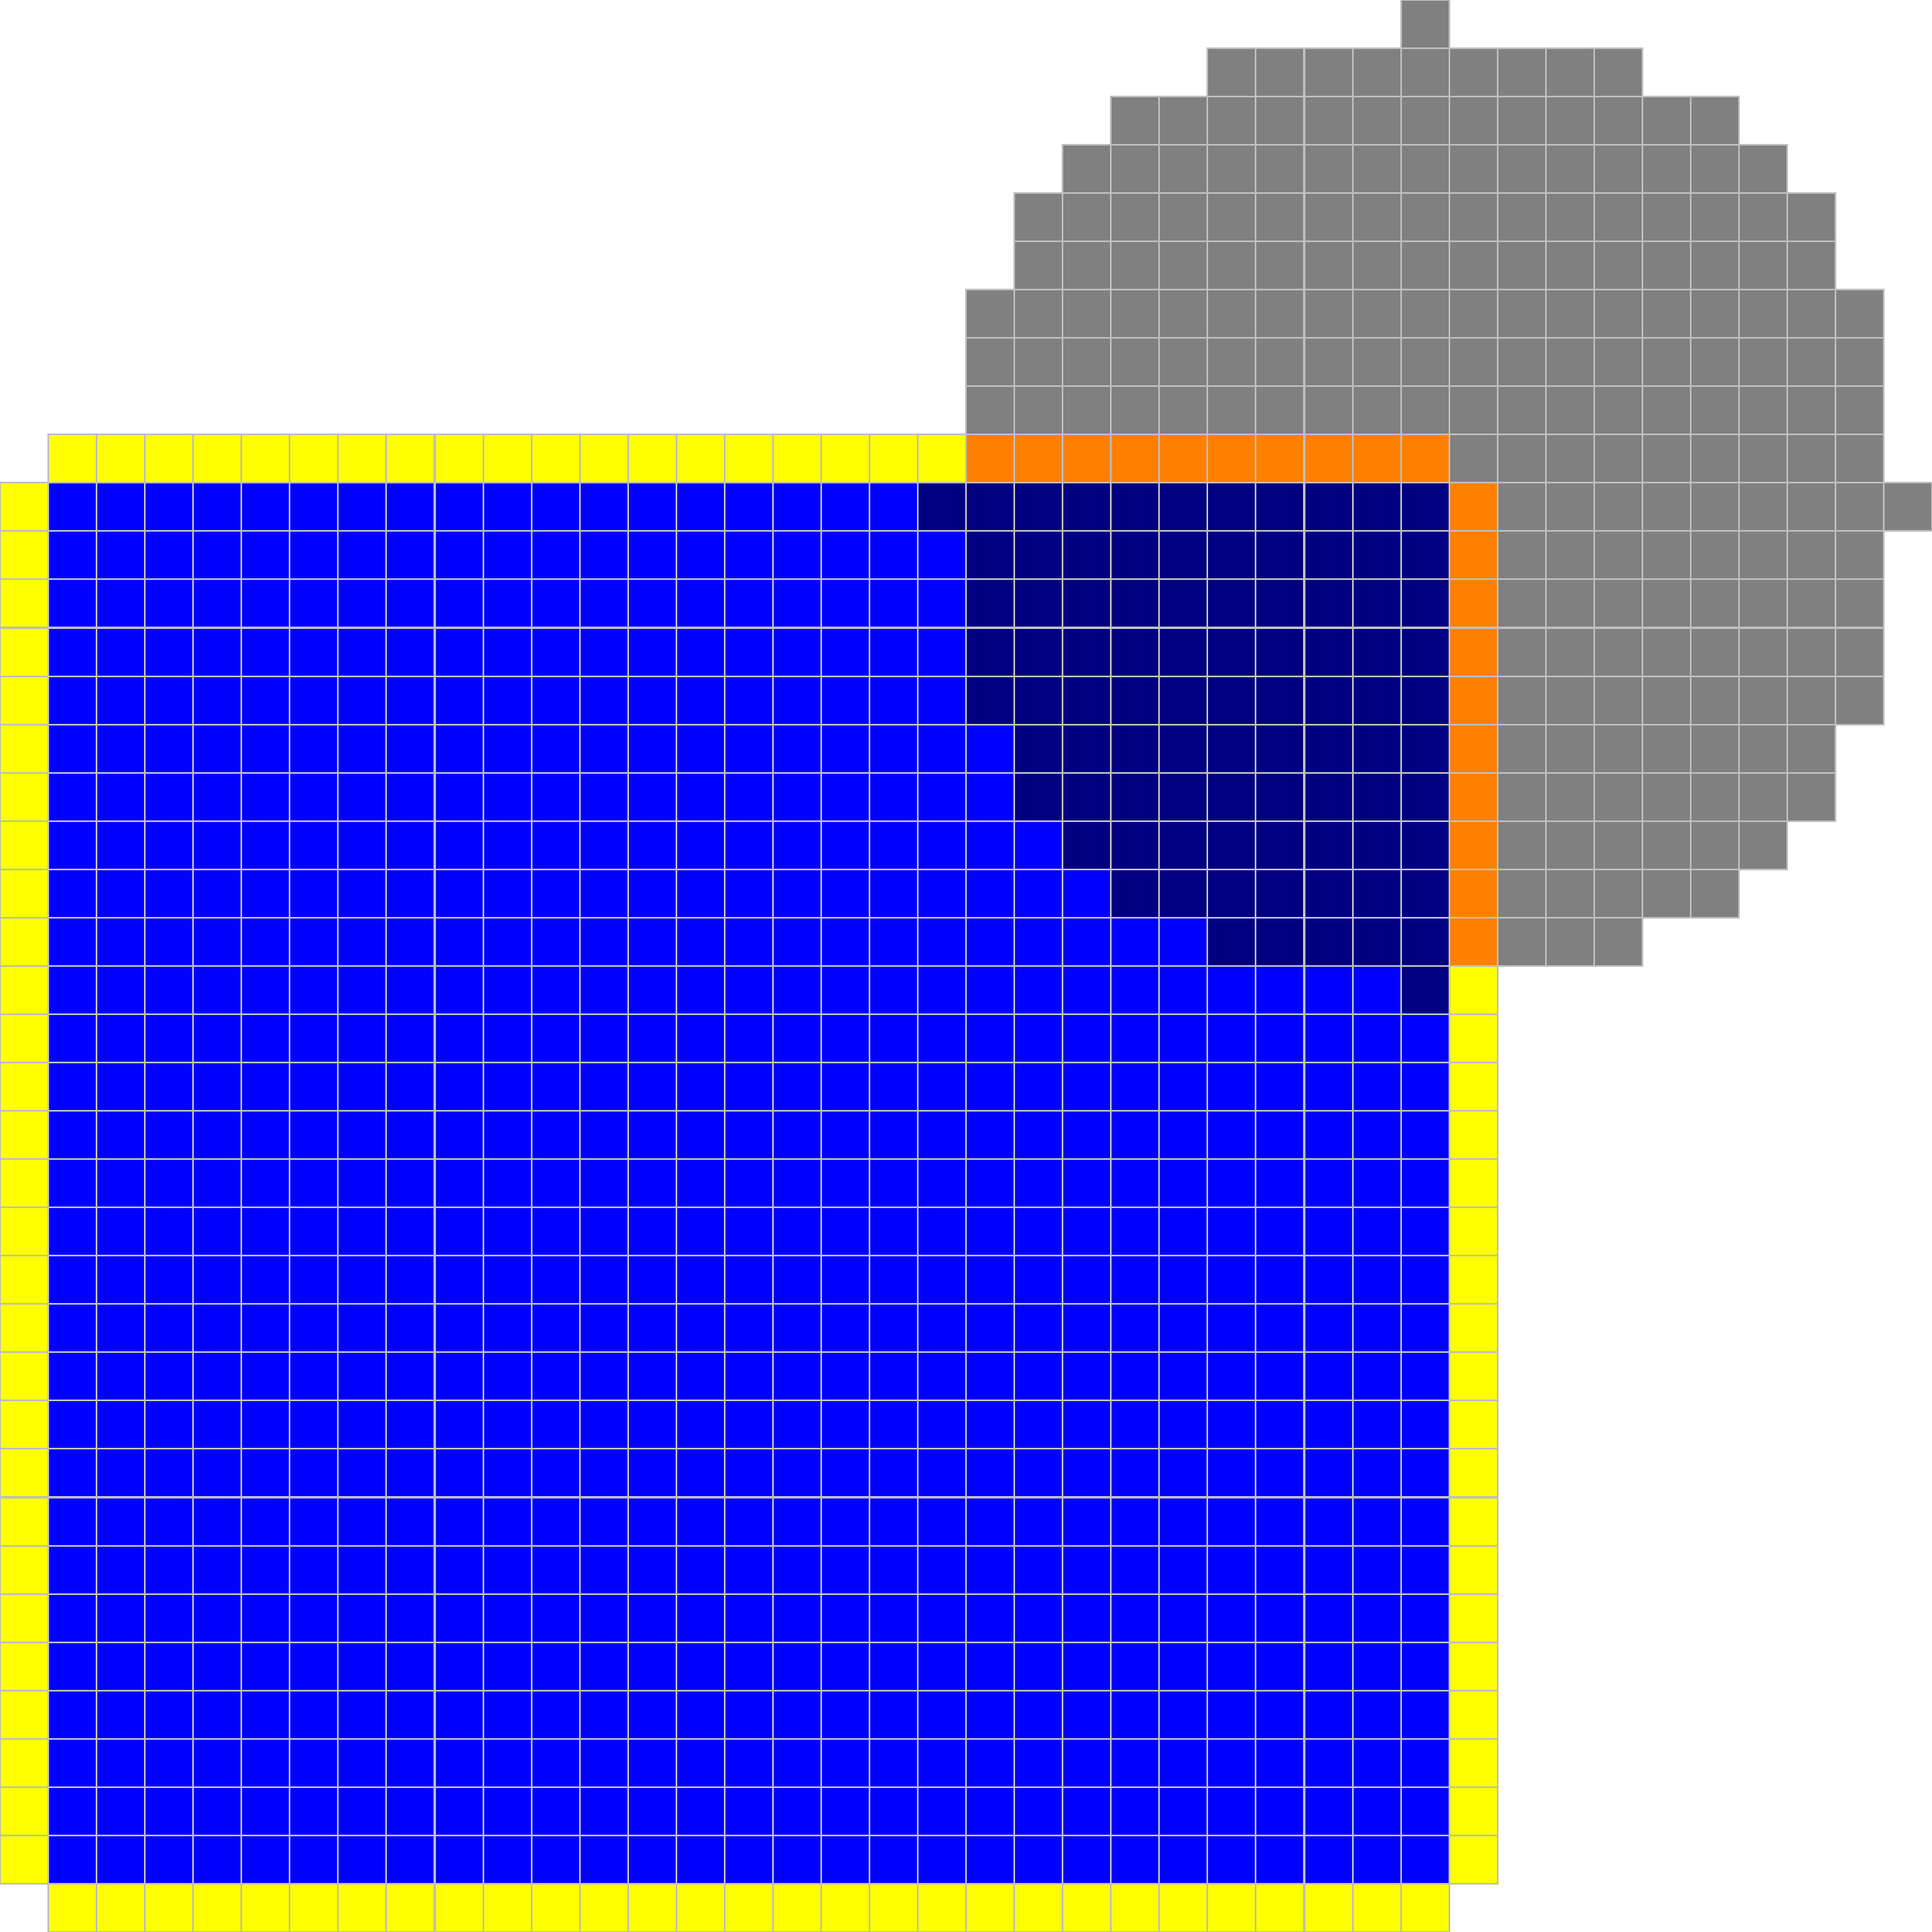
\includegraphics[scale=0.2]{figures/chapter6/contour-information/before-opt.pdf}
\label{fig:contour-info-1}
\end{minipage}%
\begin{minipage}{0.5\textwidth}
\center
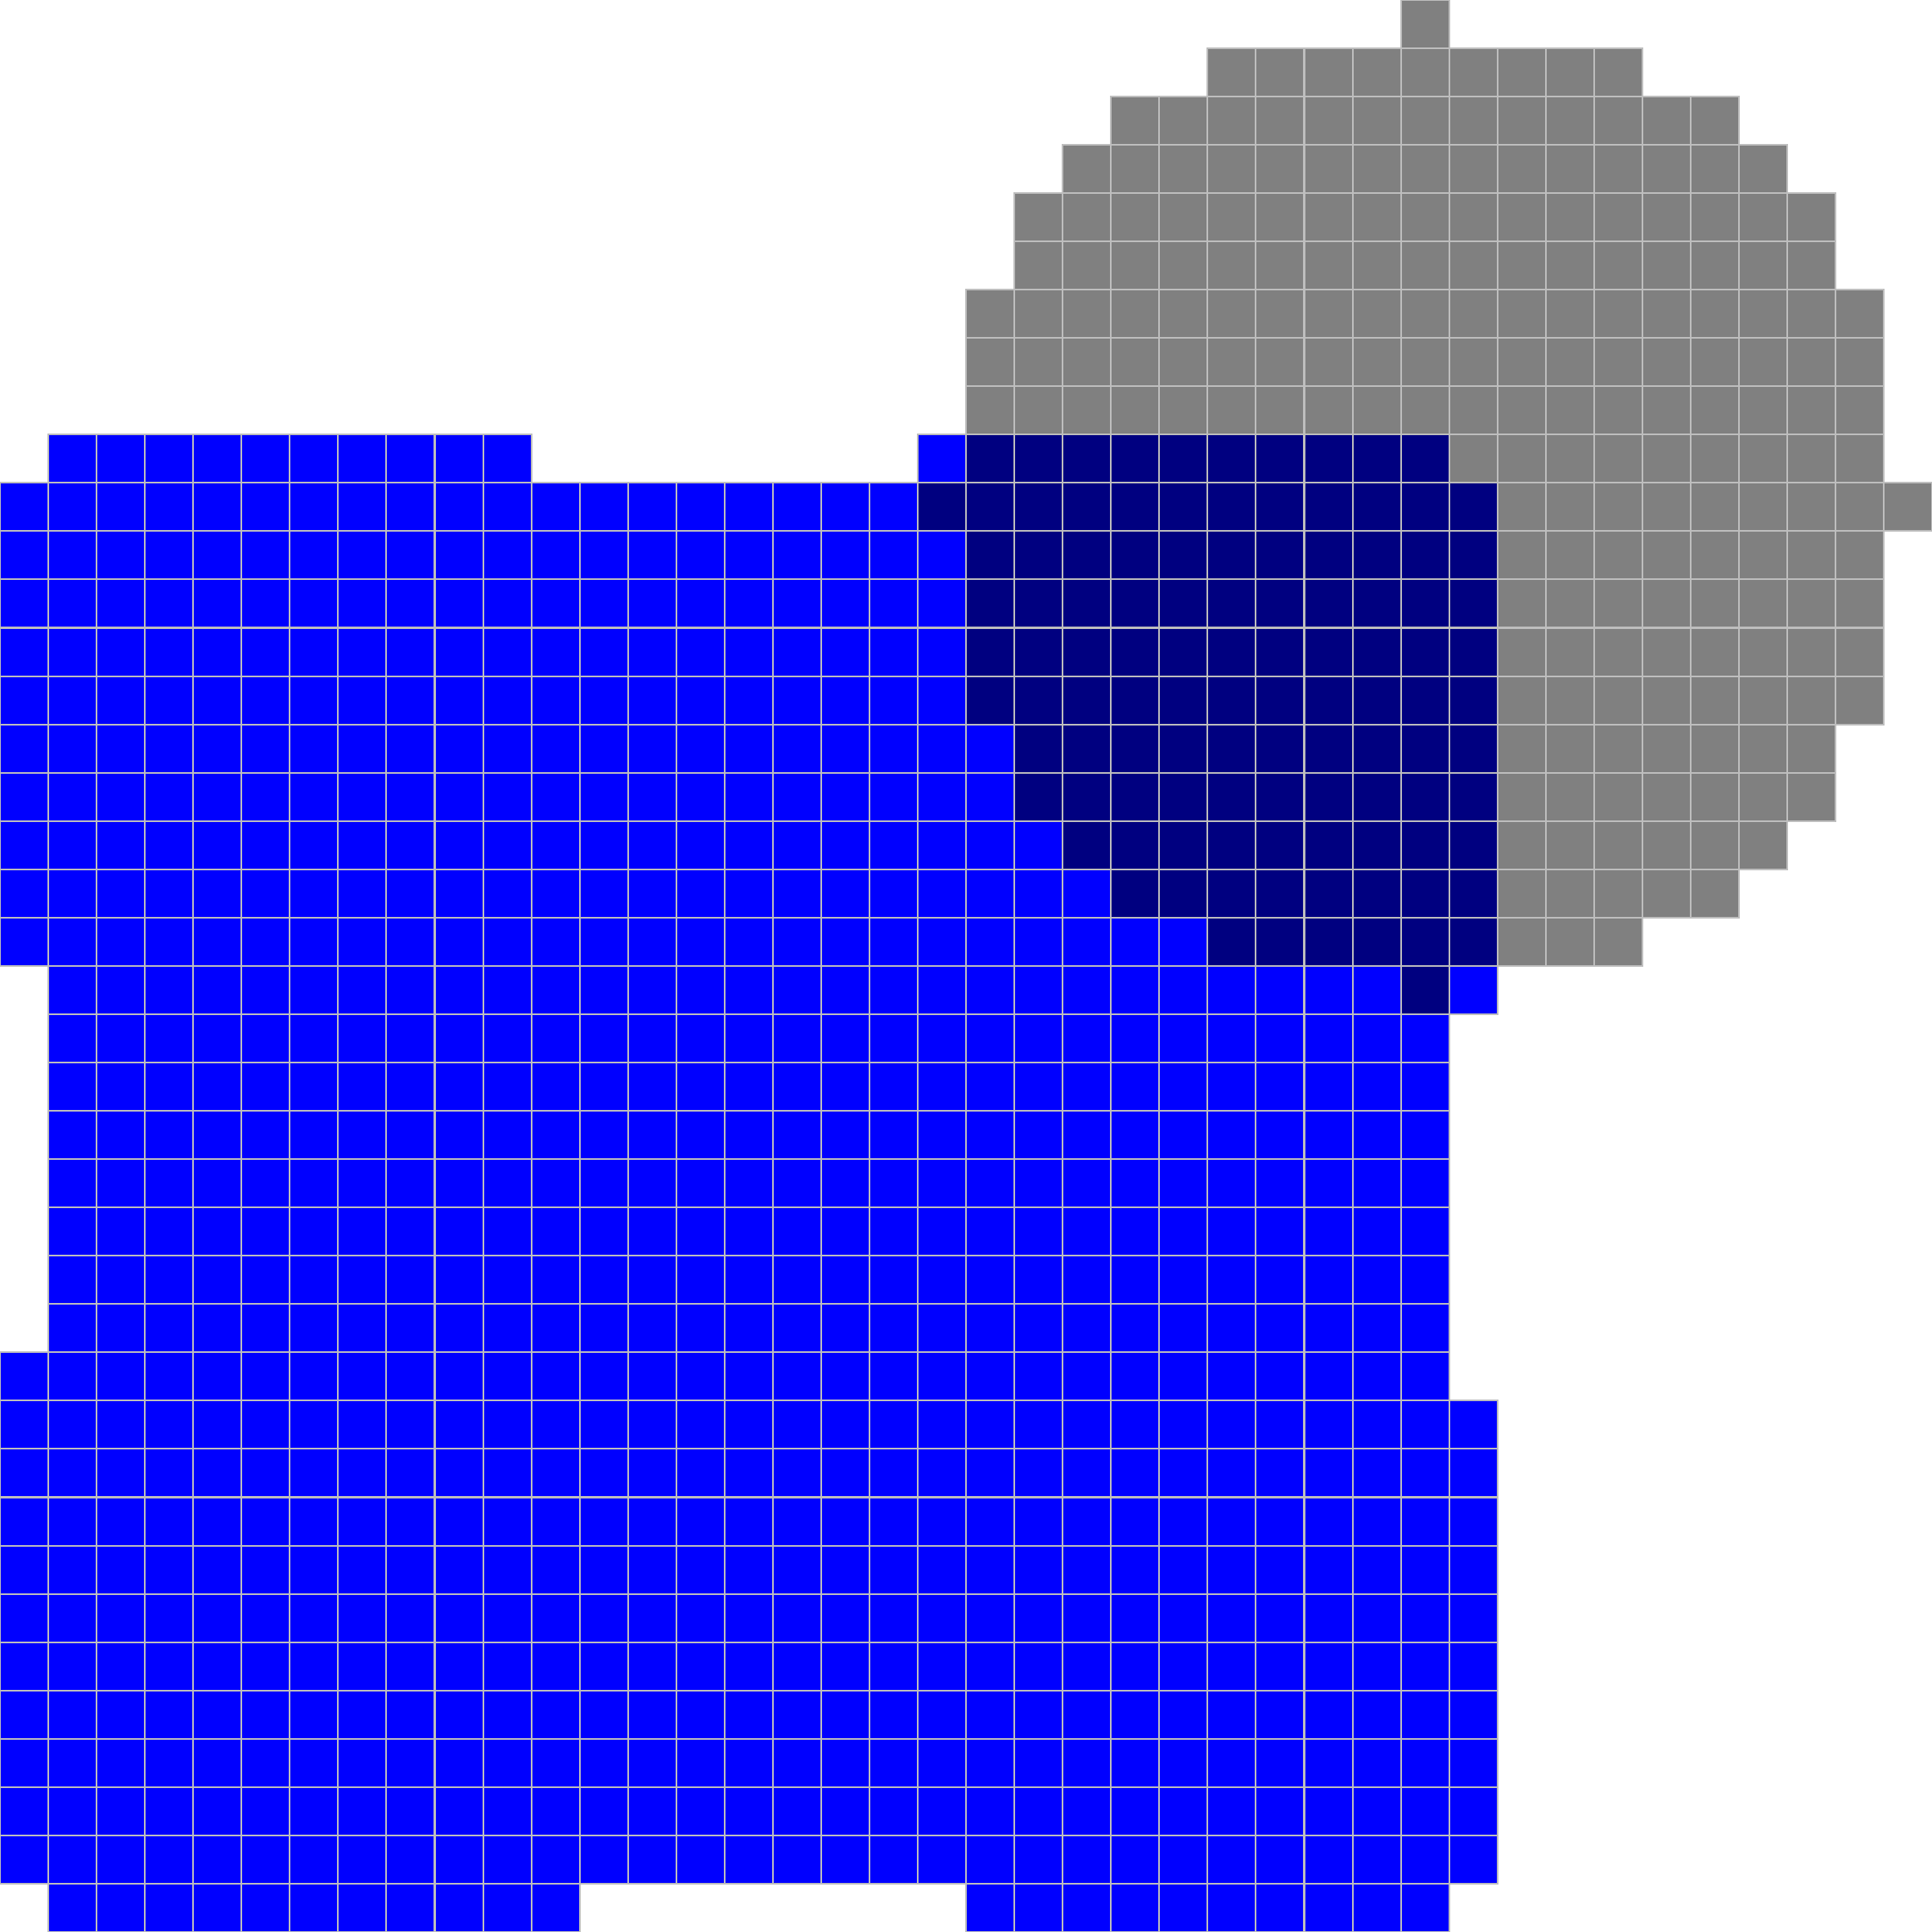
\includegraphics[scale=0.2]{figures/chapter6/contour-information/after-opt.pdf}
\label{fig:contour-info-2}
\end{minipage}%
\caption{ Directly using the optimization result of \eqref{eq:energy-family} doesn't decrease squared curvature because contour information is not present in the energy.}
\label{fig:contour-info}
\end{figure}

\begin{algorithm}
 \SetKwData{It}{i}
 \SetKwData{MIt}{maxIt}
 \SetKwData{Delta}{delta}
 \SetKwInOut{Input}{input}\SetKwInOut{Output}{output}
 \SetKwComment{comment}{//}{}
 
 \Input{A digital set $S$; The ring number $m$; Length($\alpha$), curvature($\beta$) and data($\gamma$) coefficients; the maximum number of iterations \MIt;}
 \BlankLine
 $S^{(0)} \longleftarrow S$\;
 $i \longleftarrow 1$\;
 \While{ \It $<$ \MIt  }{ 	
	\comment{Shrinking mode}
	\If{ \It is even }{	 
	 	$x^{(i)} \longleftarrow \argmin_{X^{(i)}} E_m(1-X^{(i)},S^{(i-1)})$\; 	
 		$S^{(i)} \longleftarrow F^{(i-1)} + x^{(i)}$\;
 	}
	\comment{Expansion mode} 	
 	\Else{	
	 	$x^{(i)} \longleftarrow \argmin_{X^{(i)}} E_m(1-X^{(i)},\overline{S^{(i-1)}})$\;
 		$S^{(i)} \longleftarrow \overline{ F^{(i-1)} + x^{(i)}}$\; 	
 	}
 	
	\It $\longleftarrow$ \It $+1$\;
	
 }
 \caption{Digital curvature evolution algorithm (DCE).}
 \label{alg:evolution-model}  
\end{algorithm}


As discussed in section \ref{ch6:sec:global-optimization}, the topological constraints are a fundamental part in a global optimization model for the digital elastica but the complexity added to it dampens any hope of optimizing it efficiently. In the proposed DCE model, we exclude topological constraints and we end up with the tractable binary second order energy \eqref{eq:energy-family}. However, due the lack of contour information, the minimization of \eqref{eq:energy-family} for $S^{(i)}$ results in undesirable shapes of even higher digital elastica energy values  (see figure \ref{fig:contour-info}). Interestingly, by using the inverse of the optimal assignement, we can derive a shape of lower digital elastica energy. Therefore, the next shape is given by

\begin{align*}
	S^{(i+1)} = F_{S}^{(i)} + \argmin _{}{E_m\big(1-X^{(i)},S^{(i)}} \big).
\end{align*}

Recall that the integral invariant estimator approaches curvature by computing the difference between half of the area
of a chosen ball and the area of the intersection of this ball with the shape.  In particular, regions of positive
curvature have fewer pixels in their intersection set than on its complement w.r.t the estimation ball. This implies
that variables in such regions are labeled with 1, as the unbalance grows otherwise. We attenuate curvature if we shift
the center of the estimation ball towards the interior of the shape, which means to remove the 1-labeled pixels. That is
why we take the complement of the optimization solution.


The explanation above covers the treatment of convex parts, but the way to treat concavities it's not much different. Indeed, concave regions are convex in the shape complement. The DCE algorithm \ref{alg:evolution-model} is made of two modes: shrinking and expansion. The shrinking mode handles convexities and its reasoning is explained in the last paragraph. The expansion mode operates exactly in the same way, but at the image complement, and by doing this we are able to handle
concavities. It is called expansion mode because the optimization region, in this case, is the outer pixel boundary of
the original shape. Table~\ref{tab:flow-summary} sums up these arguments.

Length and data terms should be properly defined in order to comply with the complement step of the DCE
algorithm. The length penalization is defined as

\begin{align}
  s(x_{w(p)})=\sum_{q \in \mathcal{N}_4(p)}{ t(q) }, \quad \text{where } t(q) = \left\{\begin{array}{ll}
  (x_{w(p)}-x_{w(q)})^2, & \text{if } q \in I^{(i)}\\
  (x_{w(p)}-0), & \text{if } q \in F^{(i)}\\
  (x_{w(p)}-1), & \text{otherwise }
  \end{array}\right.
  \label{eq:length-penalization}
\end{align}
	
For the moment we are not going to define any data term, as they are not important for the experiments at this section. We postpone the data term definition to chapter \ref{ch:applications}.



\begin{table}
  \center
  \setlength{\extrarowheight}{0.5em}
  \begin{tabular}{|c|c|c|c|} \hline
    shrinking mode &    $\kappa \gg 0$ & $\kappa \geq 0$ &  $\kappa < 0$ \\ \hline
    $x^{(i)}$ & $x_k=1$ & $x_k \in \{0,1\}$ & $x_k=0$ \\ \hline
    $S^{(i+1)} \leftarrow S^{(i)} - x^{(i)}$ & eroded & prob. eroded & unchanged  \\ \hline \hline
    expansion mode &    $\bar{\kappa} \gg 0$ & $\bar{\kappa} \geq 0$ & $\bar{\kappa} < 0$ \\ \hline
    $\bar{x}^{(i)}$ & $\bar{x}_k=1$ & $\bar{x}_k \in \{0,1\}$ & $\bar{x}_k=0$ \\ \hline
    $S^{(i+1)} \leftarrow \overline{\bar{S}^{(i)} - \bar{x}^{(i)}}$ & dilated & prob. dilated & unchanged \\ \hline 
  \end{tabular}
  
  \caption{  Since the curvature is negated when reversing the curve (i.e. $\bar{\kappa}=-\kappa$), this process can only shrink  convex parts in shrink mode and expand concave parts in expansion mode.}
   \label{tab:flow-summary}	  

\end{table}


In figure \ref{fig:m1-square-flow} we show the results of the DCE algorithm for $m=1,\alpha=0, \beta=1, \gamma=0$. We observe a global evolution towards rounder shapes, but several artifacts are formed along the boundary. An estimation ball of higher radius evolves the shapes faster, but the contours become noisier. Setting $\alpha >0$ attenuates the problem for lower radius but the produced shapes doens't match with our intuition of what a flow driven by the squared curvature must be like, as the evaluation of the II estimator can tell us (see figure )


Recall that at each iteration, energy \eqref{eq:energy-family} is derived by evaluating the II estimator on a fixed boundary, i.e., the contour information is not included in the optimization problem. 
Therefore, the flip of a single pixel can turn a previous negative curvature estimation in a positive one (see figure). In our current setting, this is not a desirable property. To remediate this problem we are going to evaluate the estimation balls at farther $m-rings$ of $S$. We expect to eliminate the artificats and keep a qualitative measure of the curvature for the current shape contour.


\begin{figure}
\center
\begin{tabular}{p{2.5em}ccc}
& $h=1.0$ & $h=0.5$ & $h=0.25$ \\[2em]
\multirow{2}{*}{$\alpha=0$}& 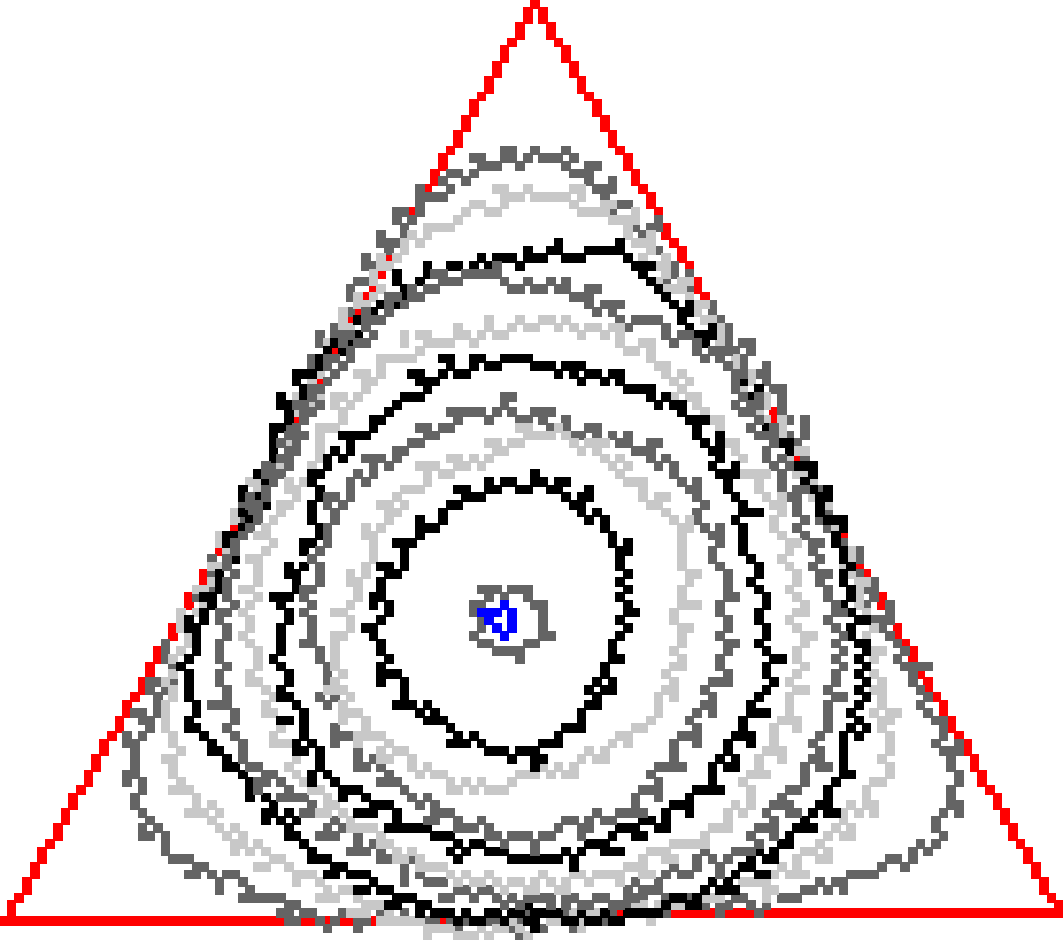
\includegraphics[scale=0.25]{figures/chapter6/radius-effect/triangle/improve/len_pen0/radius-3/summary.pdf} &
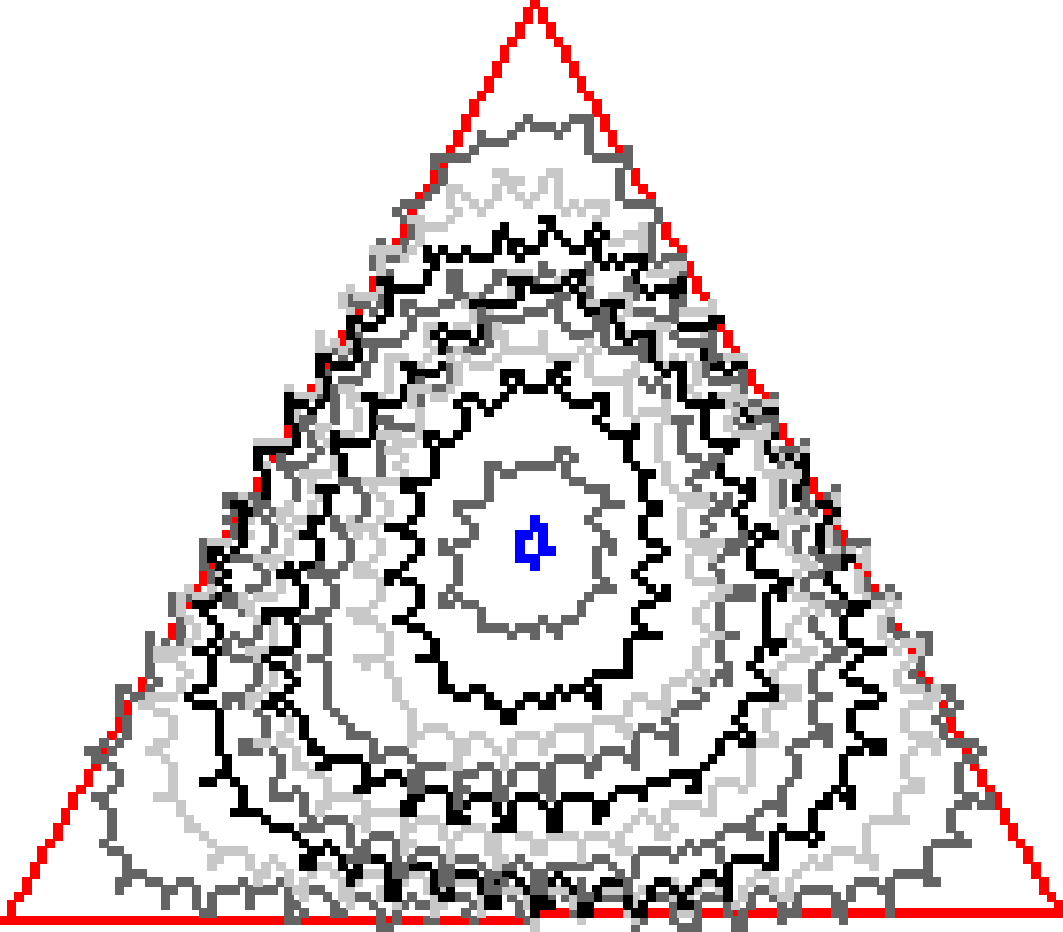
\includegraphics[scale=0.24]{figures/chapter6/radius-effect/triangle/improve/len_pen0/radius-5/summary.pdf} &
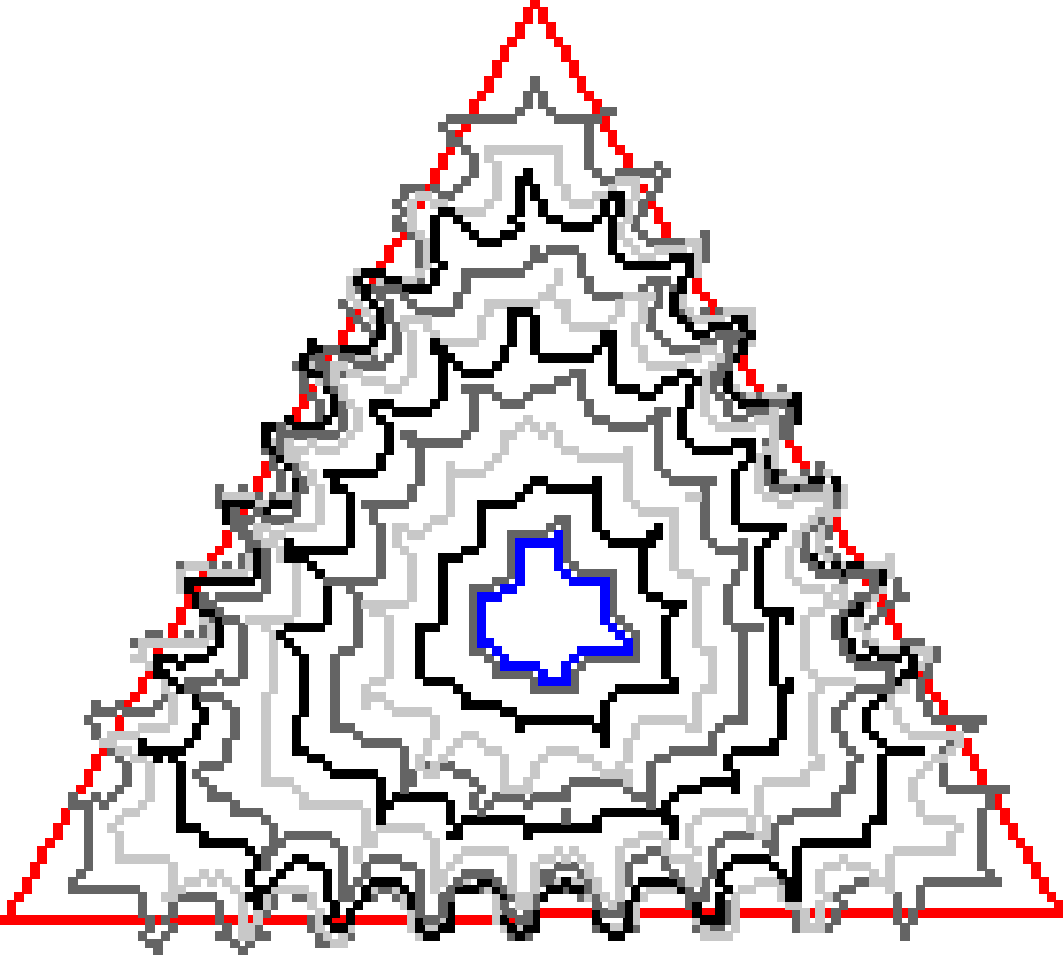
\includegraphics[scale=0.24]{figures/chapter6/radius-effect/triangle/improve/len_pen0/radius-9/summary.pdf} \\[2em]
& 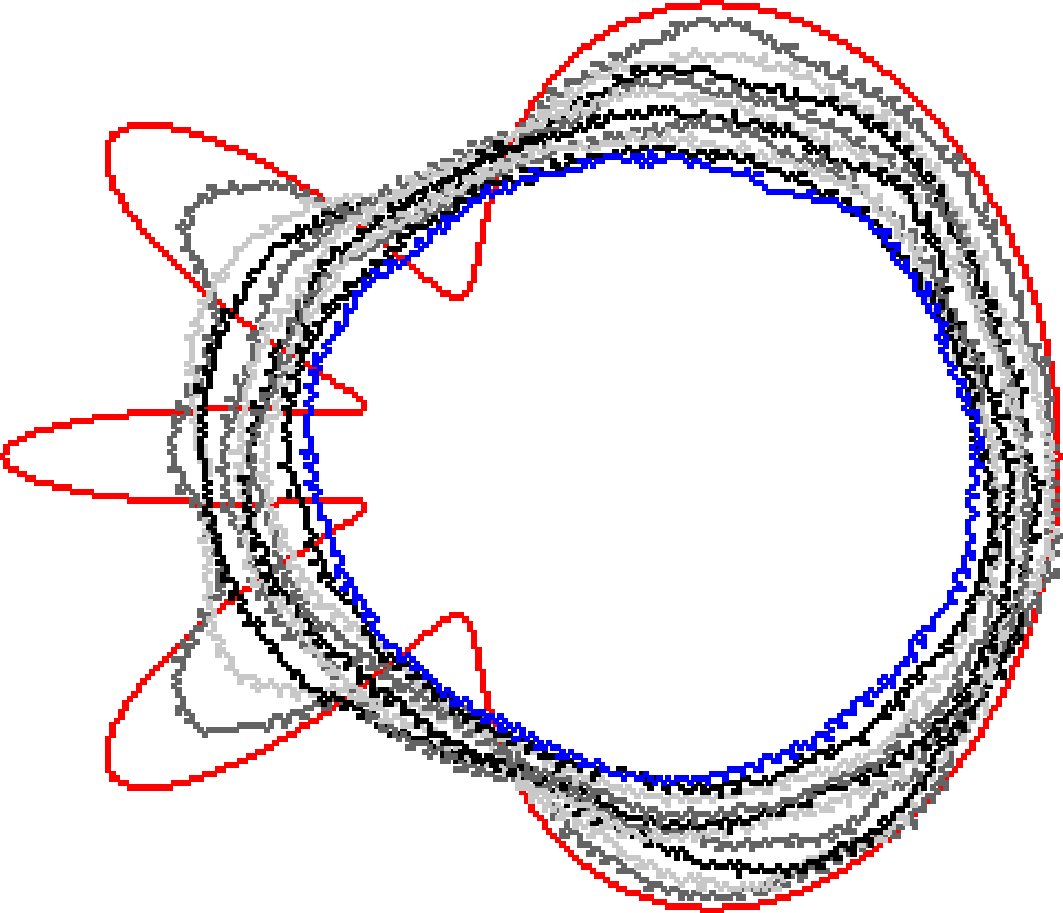
\includegraphics[scale=0.24]{figures/chapter6/radius-effect/flower/improve/len_pen0/radius-3/summary.pdf} &
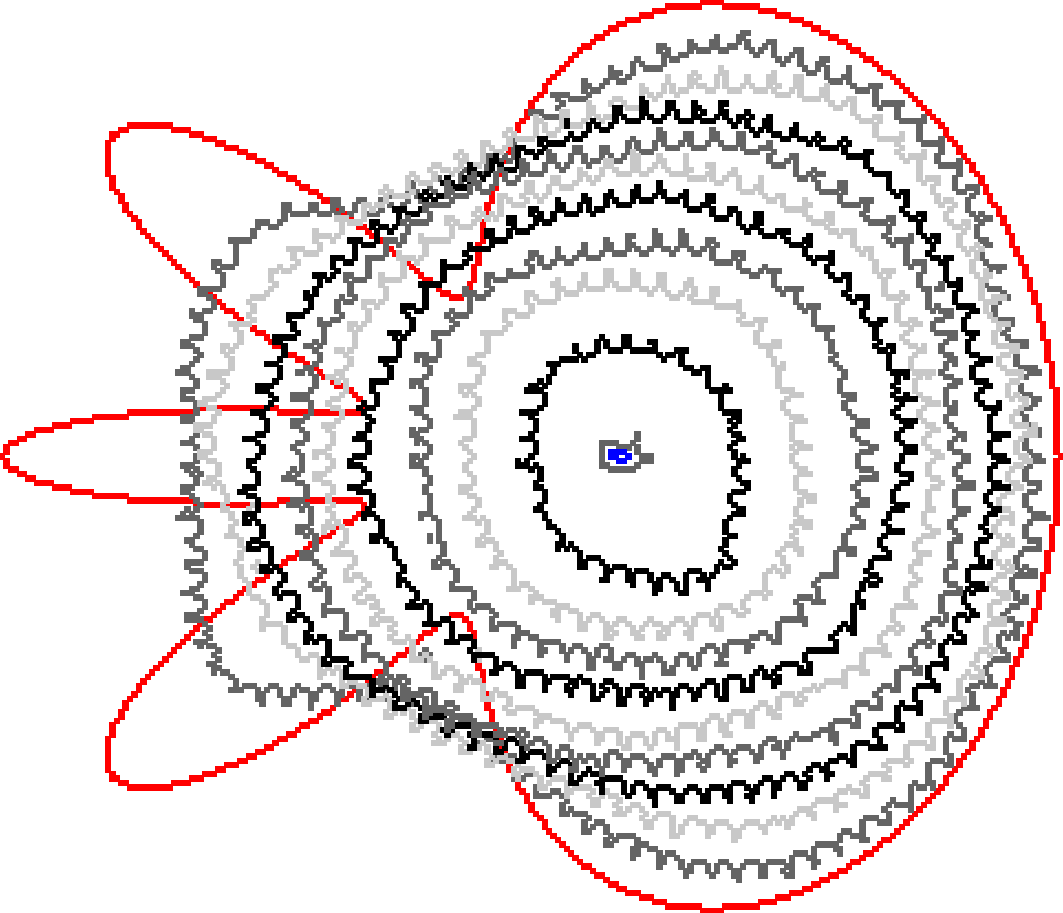
\includegraphics[scale=0.24]{figures/chapter6/radius-effect/flower/improve/len_pen0/radius-5/summary.pdf} &
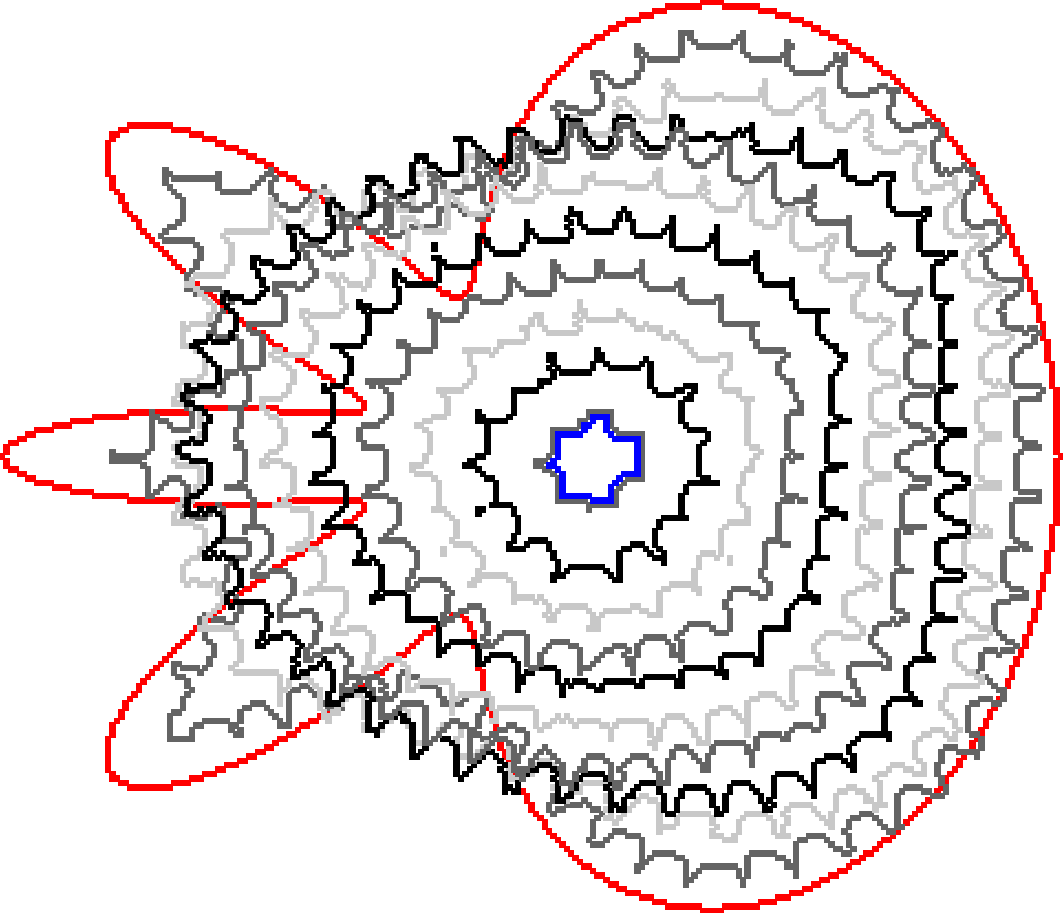
\includegraphics[scale=0.24]{figures/chapter6/radius-effect/flower/improve/len_pen0/radius-9/summary.pdf} \\
\hline \\
\multirow{2}{*}{$\alpha=0.5$}& 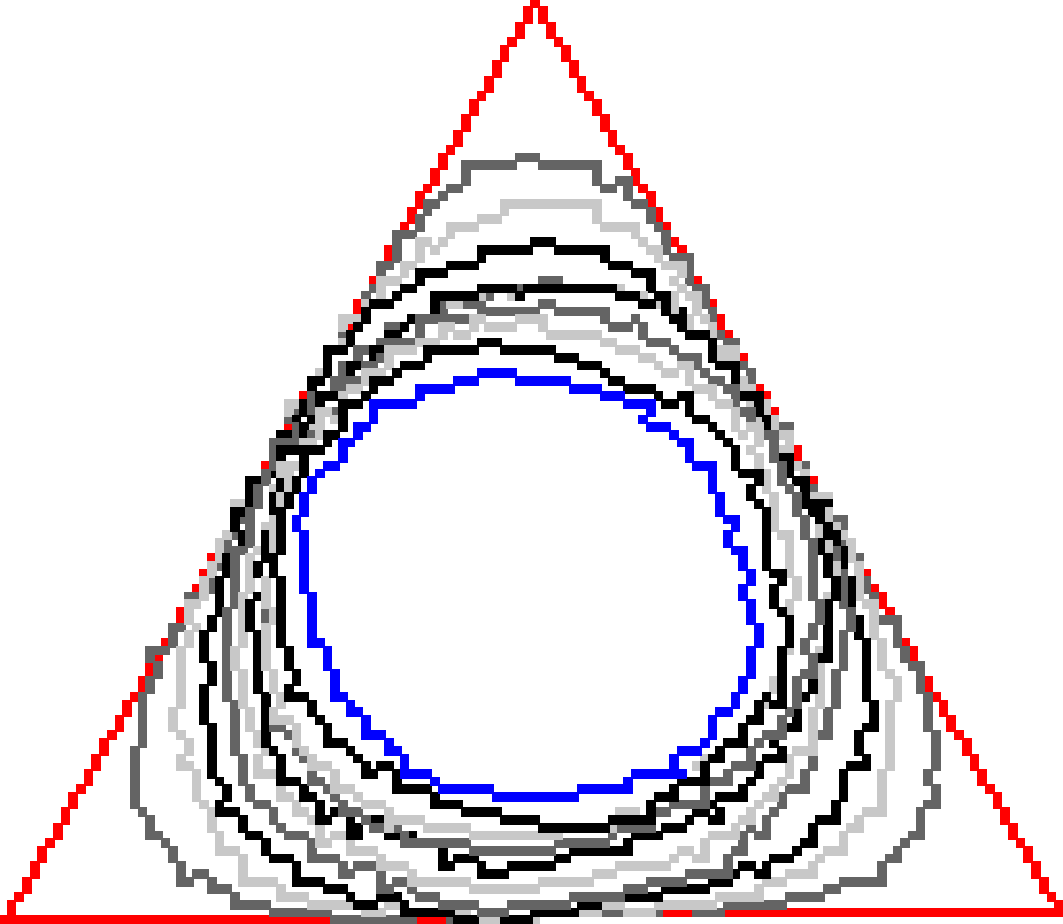
\includegraphics[scale=0.25]{figures/chapter6/radius-effect/triangle/improve/len_pen0.5/radius-3/summary.pdf} &
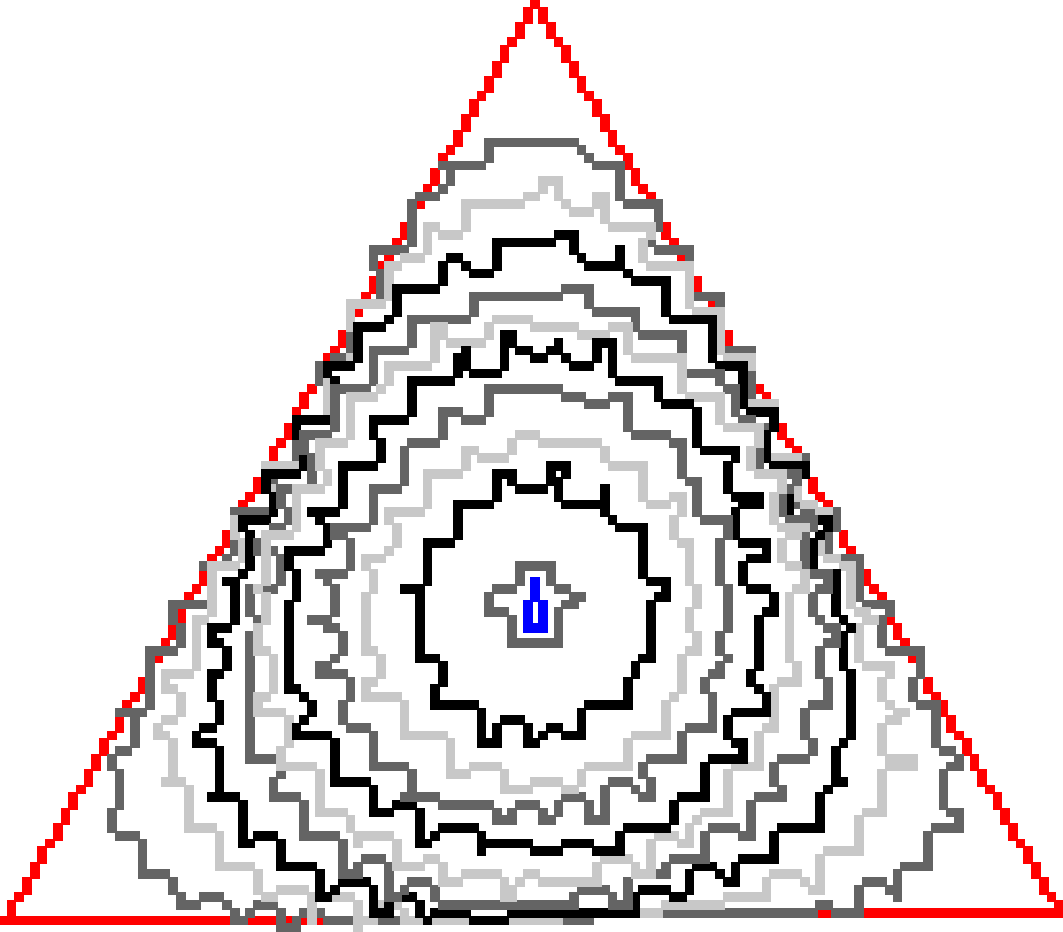
\includegraphics[scale=0.24]{figures/chapter6/radius-effect/triangle/improve/len_pen0.5/radius-5/summary.pdf} &
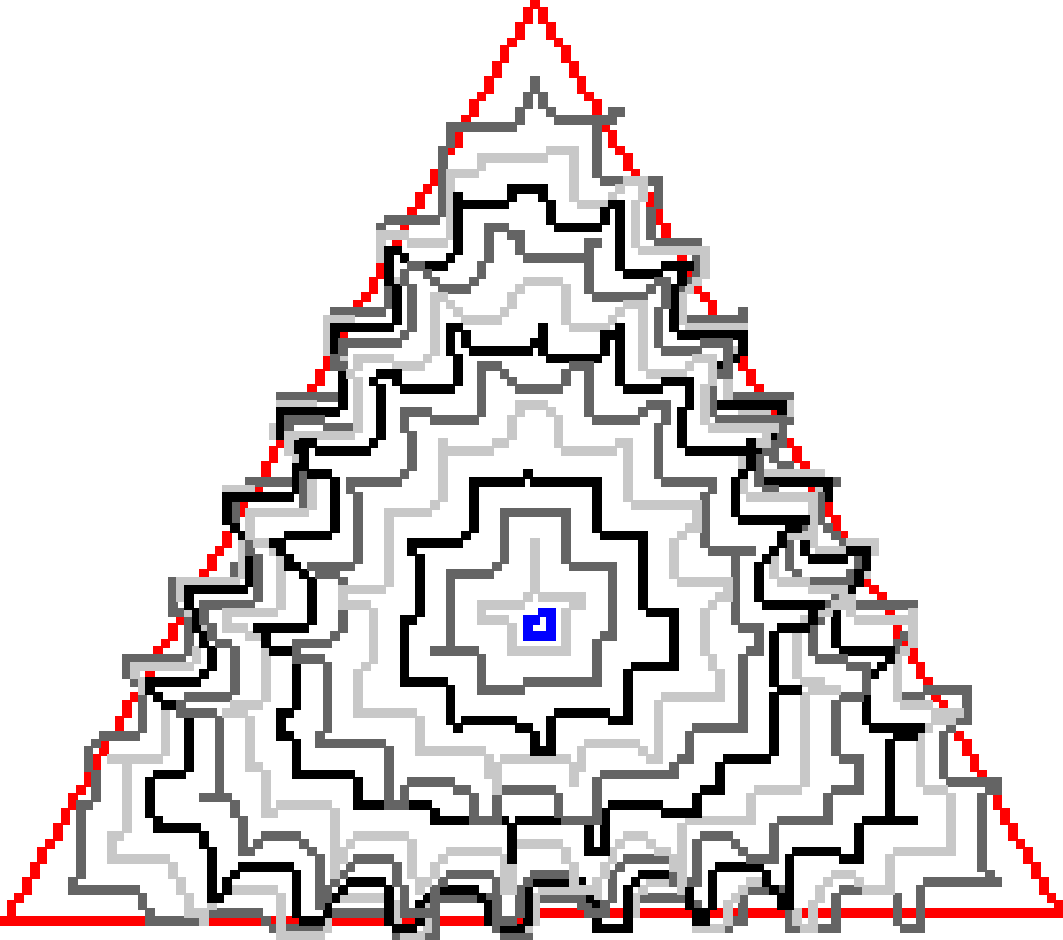
\includegraphics[scale=0.24]{figures/chapter6/radius-effect/triangle/improve/len_pen0.5/radius-9/summary.pdf} \\[2em]
& 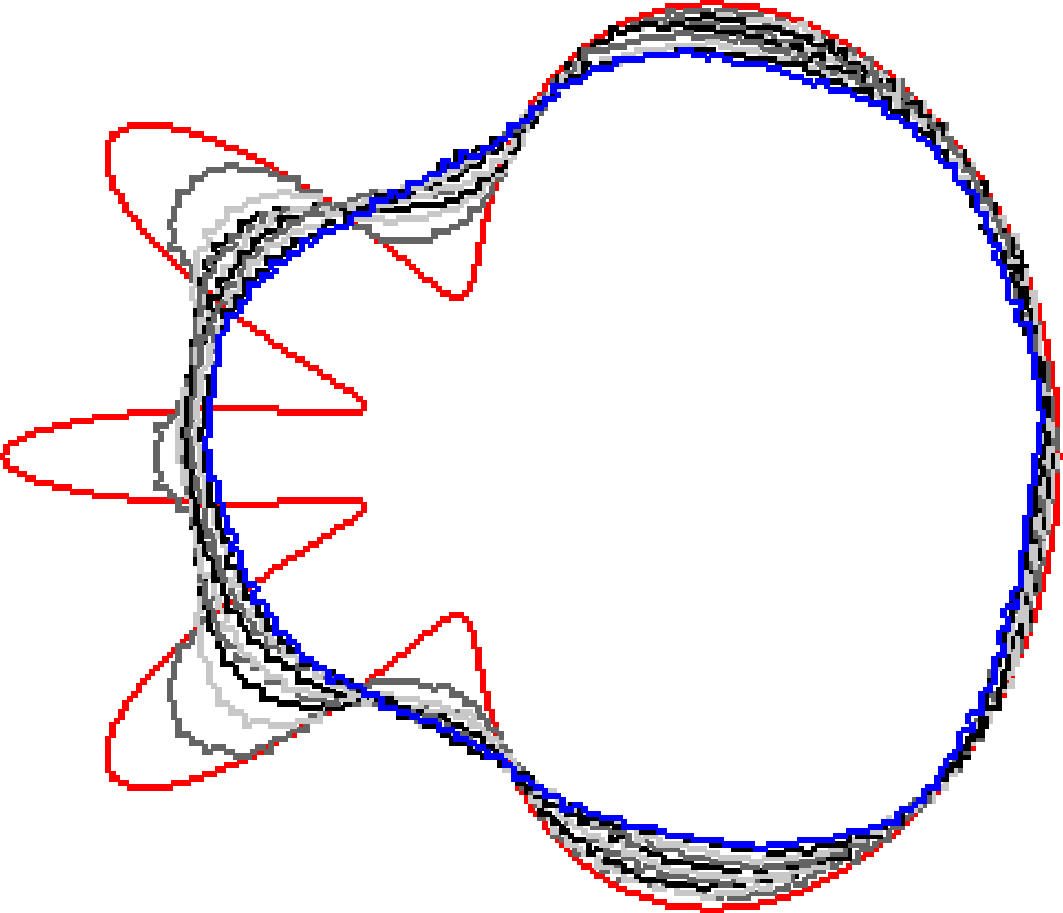
\includegraphics[scale=0.24]{figures/chapter6/radius-effect/flower/improve/len_pen0.5/radius-3/summary.pdf} &
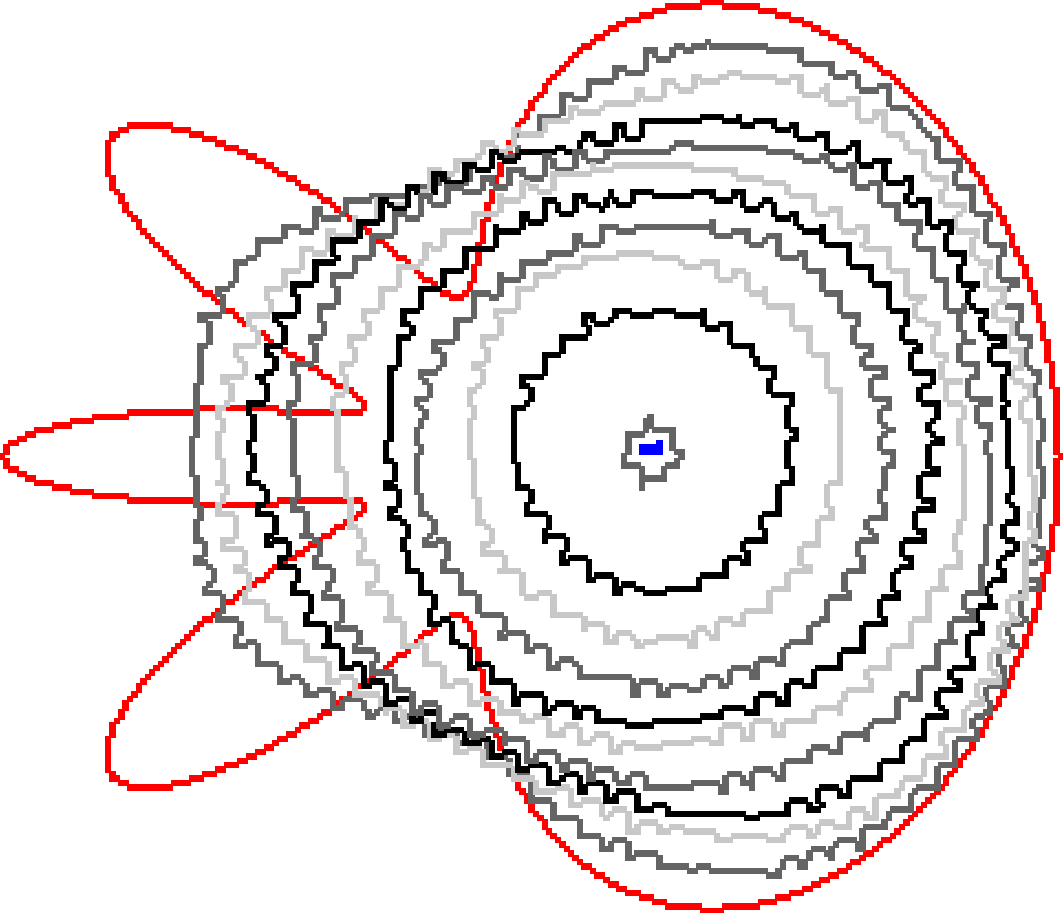
\includegraphics[scale=0.24]{figures/chapter6/radius-effect/flower/improve/len_pen0.5/radius-5/summary.pdf} &
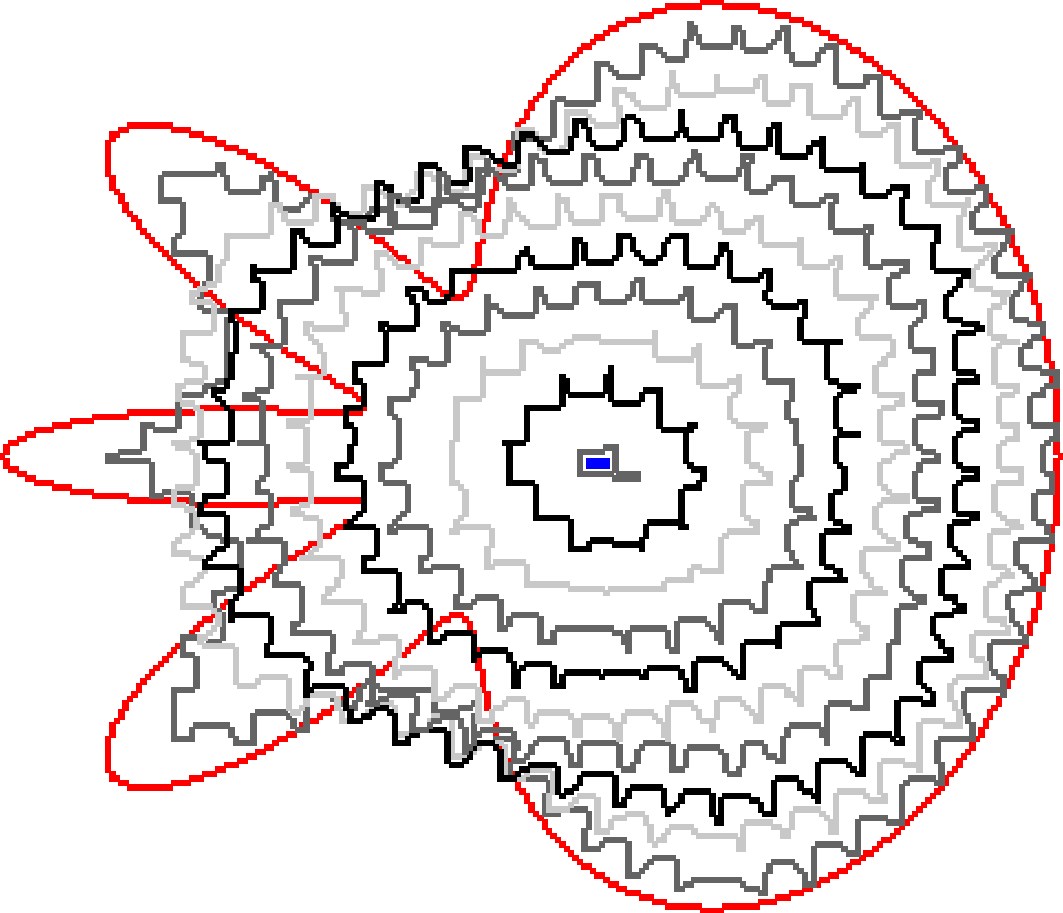
\includegraphics[scale=0.24]{figures/chapter6/radius-effect/flower/improve/len_pen0.5/radius-9/summary.pdf}
\end{tabular}

\caption{The algorithm is very sensitive to the little variations of the estimator, which are particularly important in regions of low squared curvature. Artifacts are somewhat reduced with a length penalization but increases if we use a higher ball radius. }
\label{fig:m1-square-flow}
\end{figure}


\begin{figure}
\center
\subfloat[]{
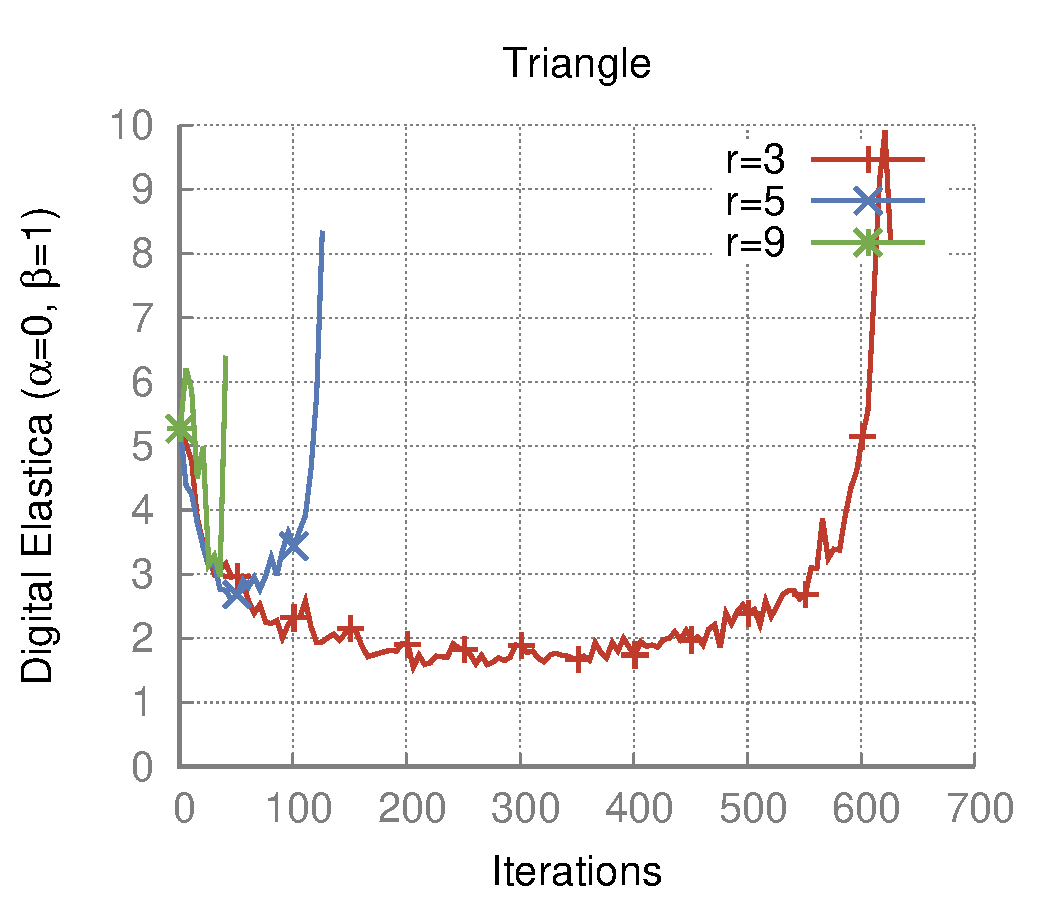
\includegraphics[scale=0.45]{figures/chapter6/radius-effect/triangle/improve/len_pen0/radius-3/radius-effect.pdf}}%
\subfloat[]{
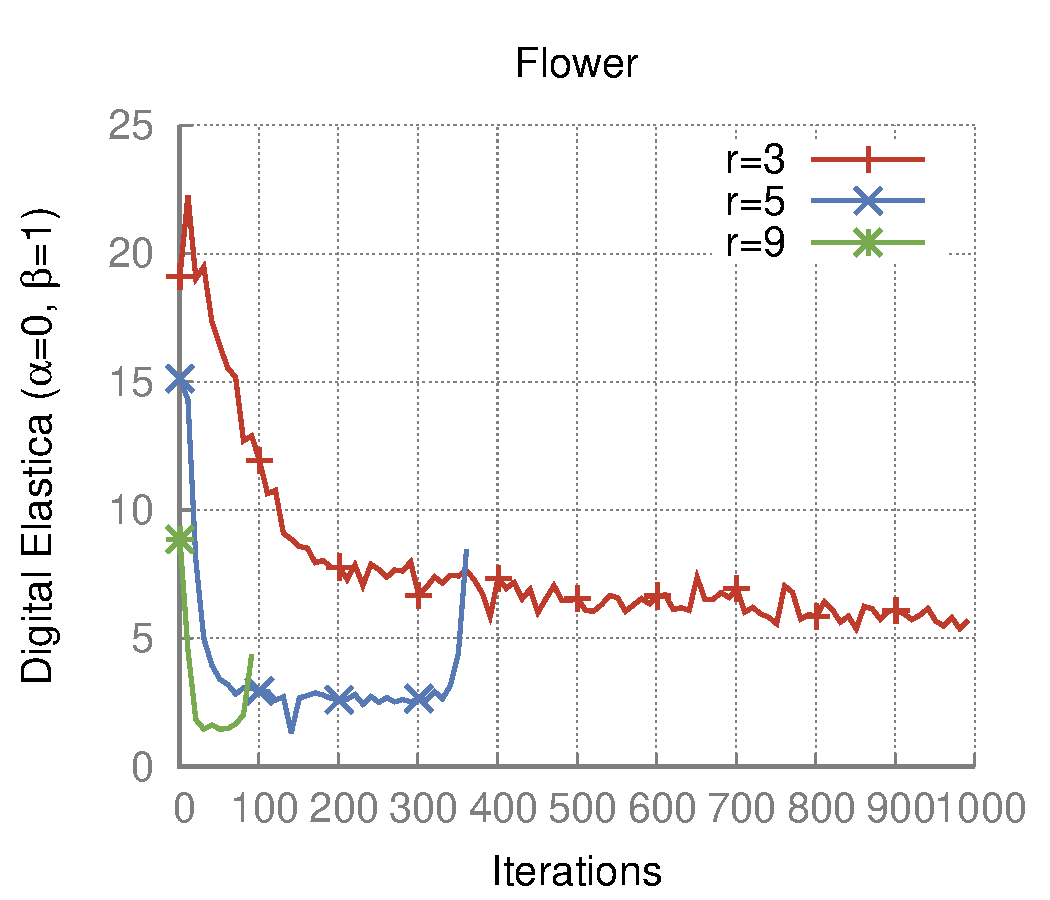
\includegraphics[scale=0.45]{figures/chapter6/radius-effect/flower/improve/len_pen0/radius-3/radius-effect.pdf}}%
\caption{The digital elastica decreases in a turbulent way.}
\end{figure}


\section{Artifacts elimination}

In the previous section we noticed that the algorithm produces shapes with many artifacts due to the small uncertainties
of the estimator along regions of low squared curvature. We argue that, by evaluating the estimation ball along outer
ring sets we avoid those sensitive areas by focusing the optimization process only on regions with highest squared
curvature value.

In figure \ref{} we evaluate several flows for different energies $E_m$. As expected, the number of artifacts decrease as the value of $m$ increases. We confirm the stability of the model by looking at the plots of the digital elastica energy values for the produced shapes.





%\begin{figure}[]
%\center
%\center
%\begin{minipage}[b]{0.33\textwidth}
%	\subfloat[$r=5, m=1$\label{}]{%
%	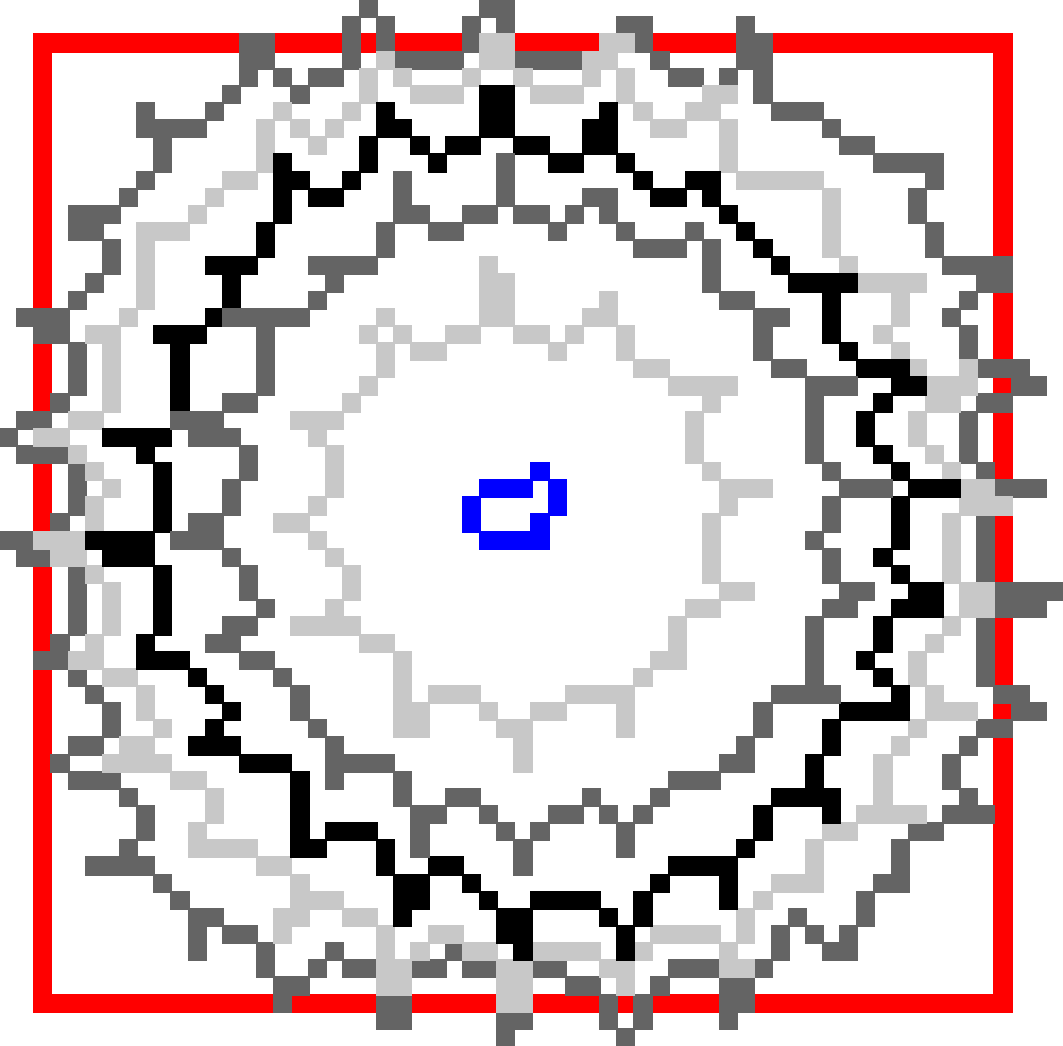
\includegraphics[scale=0.2]{figures/chapter6/farther-rings/square-r5-l1/summary_flow.pdf}
%	}%
%\end{minipage}%
%\begin{minipage}[b]{0.33\textwidth}
%	\subfloat[$r=5, m=3$\label{}]{%
%	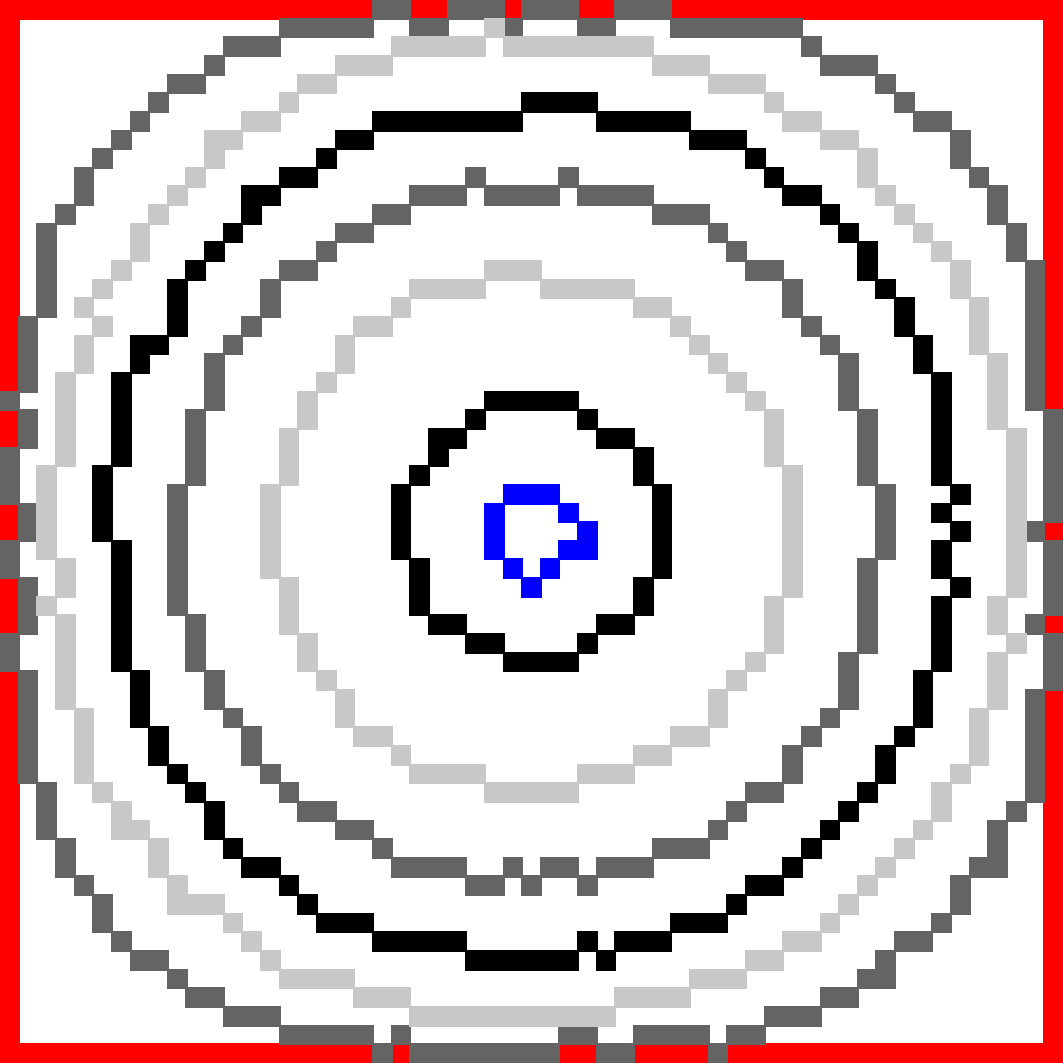
\includegraphics[scale=0.2]{figures/chapter6/farther-rings/square-r5-l3/summary_flow.pdf}
%	}%
%\end{minipage}%
%\begin{minipage}[b]{0.33\textwidth}
%	\subfloat[$r=5, m=5$\label{}]{%
%	\includegraphics[scale=0.2]{figures/chapter6/farther-rings/square-r5-l5/summary_flow.pdf}
%	}%
%\end{minipage}%
%\caption{By positioning the estimation ball on farther rings, we minimize artifacts creation. \label{fig:mx-square-flow}}
%\end{figure}

In our experiments, the best results are obtained by executing DCE algorithm with $m$ equal to $r$, where $r$ is
  the estimation ball radius (see figure \ref{fig:mx-square-flow}). We observe that digital elastica may increase after some
  iterations if chosen radius is too large, as in the case of the triangle in figure \ref{fig:mx-flow-gs-radius-effect}
  in which the flow converges to a single point. We conjecture that an appropriated value for the radius should be given
  by the shape reach.  The produced flow has no difficulties in handling changes on topology, and it presents different
  speeds for regions with low and high curvature values, as illustrated in figure
  \ref{fig:mx-speed-variation-hole-filling}.

%\begin{figure}
%\center				
%		\setcounter{subfigure}{-3}
%		\subfloat[$r=3,h=0.5$]{%
%		\subfloat{%
%		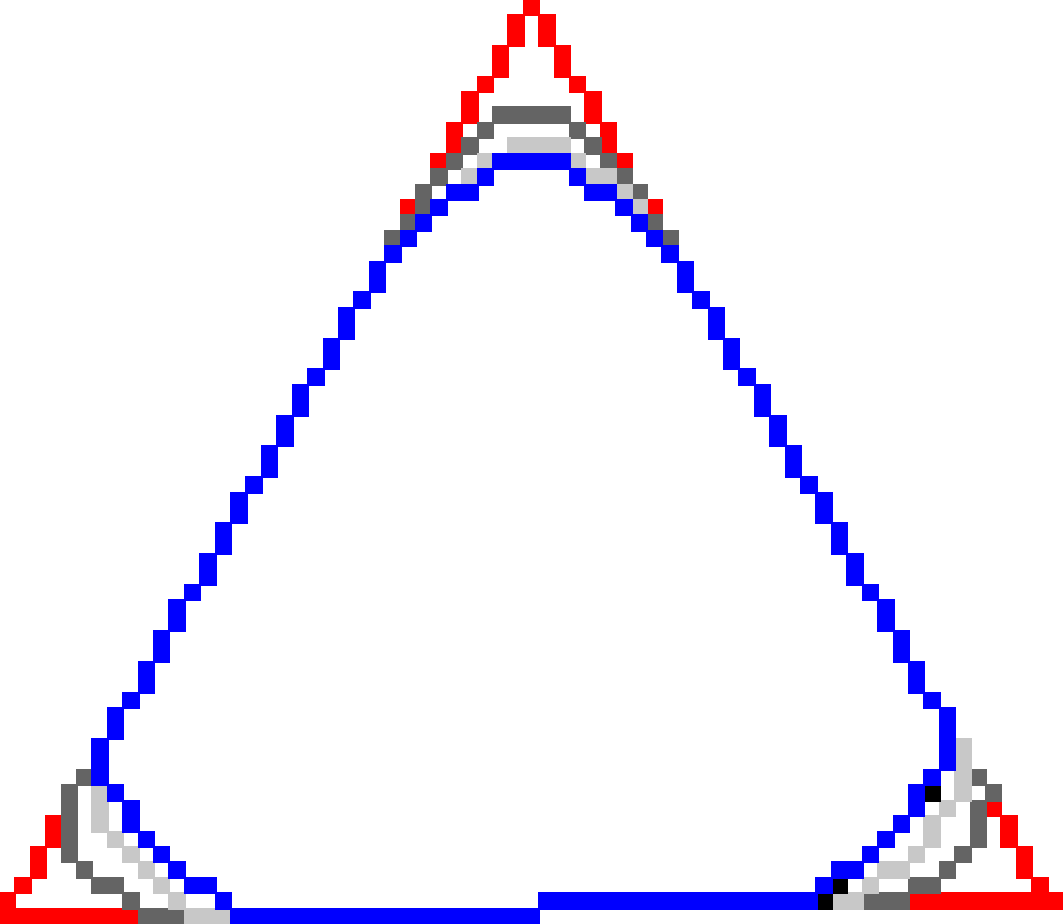
\includegraphics[scale=0.2]{figures/chapter6/grid-radius-effect/triangle/r3-h0.5/summary_flow.pdf}
%		}%
%		\hspace{15pt}
%		\subfloat{%
%		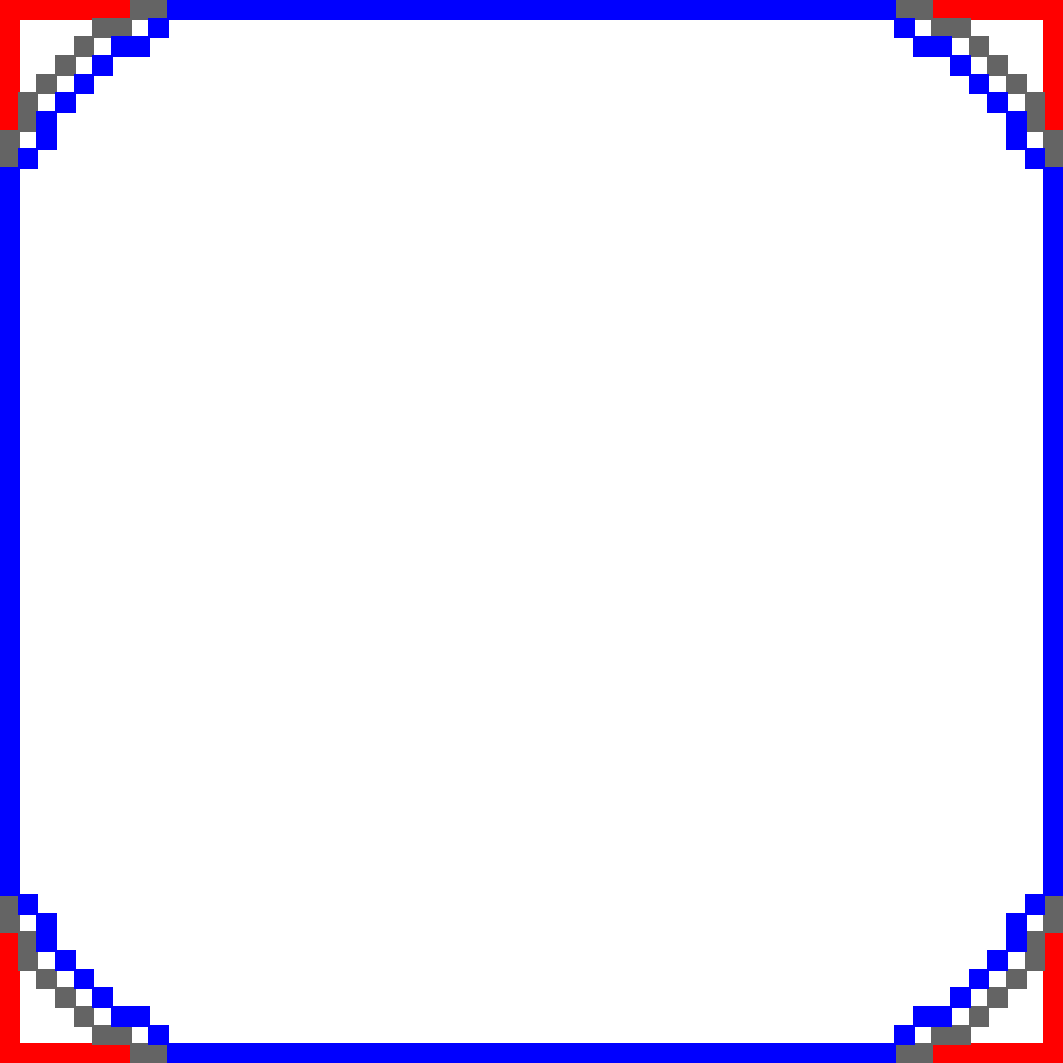
\includegraphics[scale=0.15]{figures/chapter6/grid-radius-effect/square/r3-h0.5/summary_flow.pdf}}%
%		\hspace{15pt}
%		\subfloat{%
%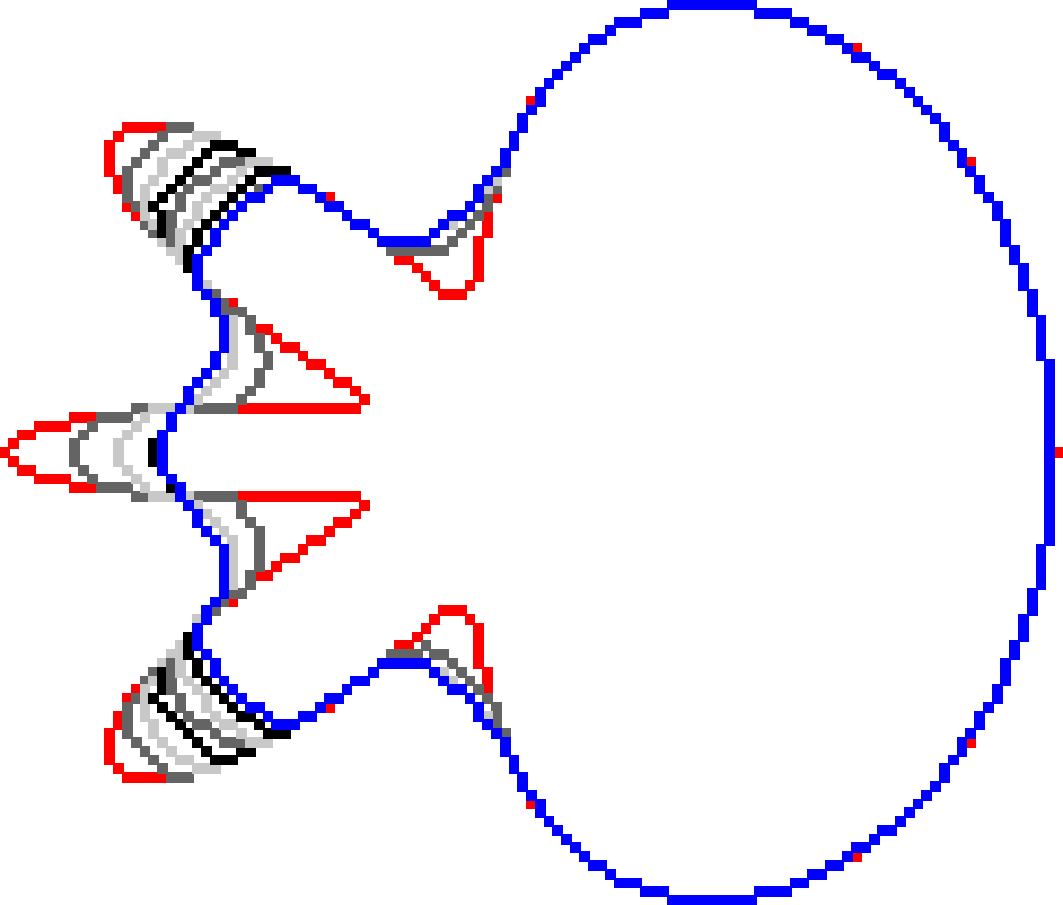
\includegraphics[scale=0.2]{figures/chapter6/grid-radius-effect/flower/r3-h0.5/summary_flow.pdf}}%
%		}		
%	
%		\setcounter{subfigure}{-2}
%		\subfloat[$r=5,h=0.5$]{%
%		\subfloat{%
%		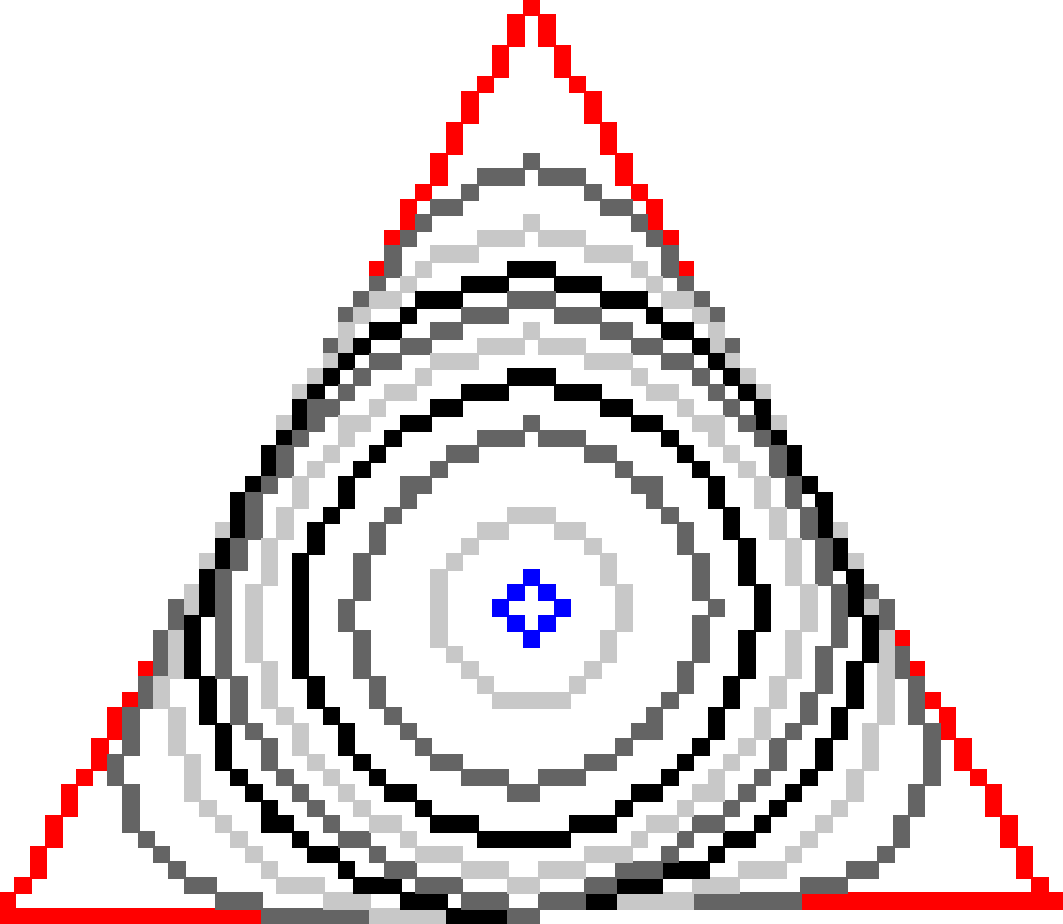
\includegraphics[scale=0.2]{figures/chapter6/grid-radius-effect/triangle/r5-h0.5/summary_flow.pdf}
%		}%1
%		\hspace{15pt}
%		\subfloat{%
%		\includegraphics[scale=0.15]{figures/chapter6/grid-radius-effect/square/r5-h0.5/summary_flow.pdf}}%
%		\hspace{15pt}
%		\subfloat{%
%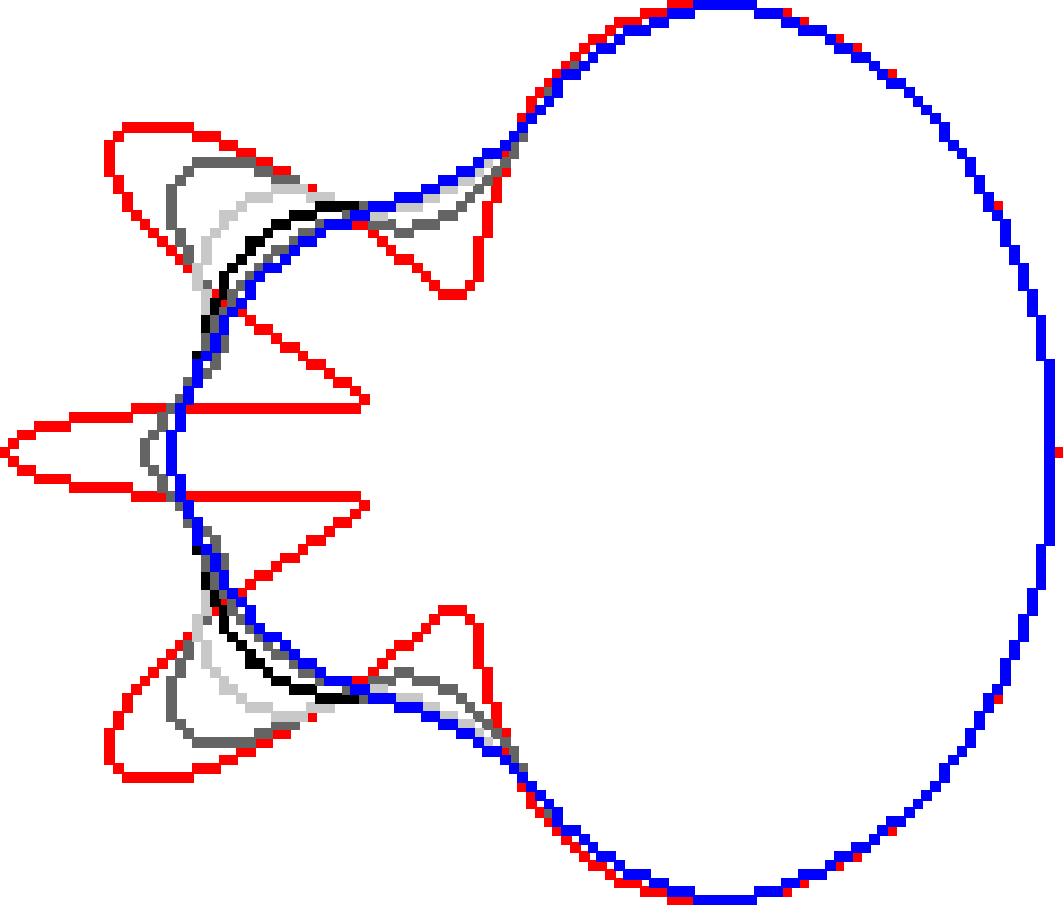
\includegraphics[scale=0.2]{figures/chapter6/grid-radius-effect/flower/r5-h0.5/summary_flow.pdf}}%
%		}\\
%		\subfloat[Digital elastica evaluation ($r=5,h=0.5$)]{%
%		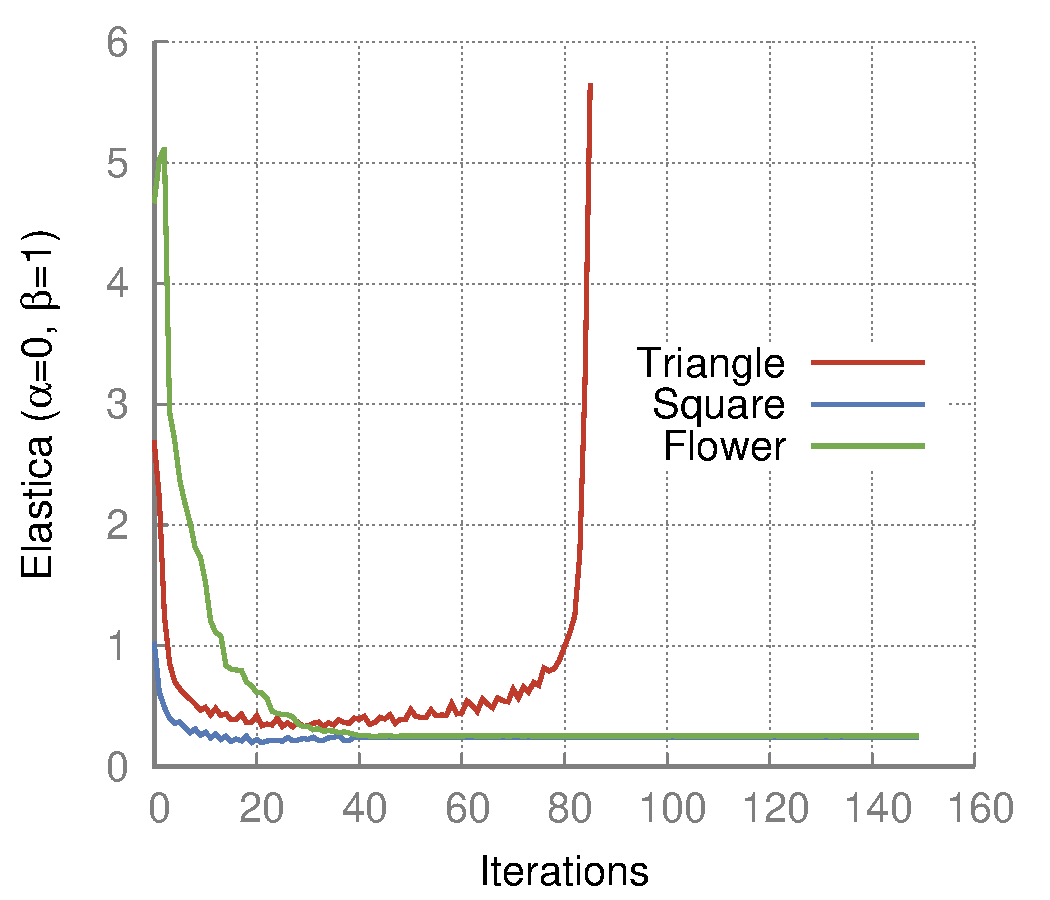
\includegraphics[scale=0.5]{figures/chapter6/elastica-energy-plot/square-flower-triangle.pdf}						
%		}
%\caption{The choice of radius impacts the flow. In the figures, the flow ceases to evolve for all shapes  when $r=3$ (a). In figure (b), for $r=5$, the triangle evolves to a single point, while the others stop  in an intermediate shape, as in (a). In figure (c), we observe that for a given choice of radius, the digital elastica may increase after a certain number of iterations. }
%\label{fig:mx-flow-gs-radius-effect}
%\end{figure}


%\begin{figure}
%\center
%\subfloat[]{%
%	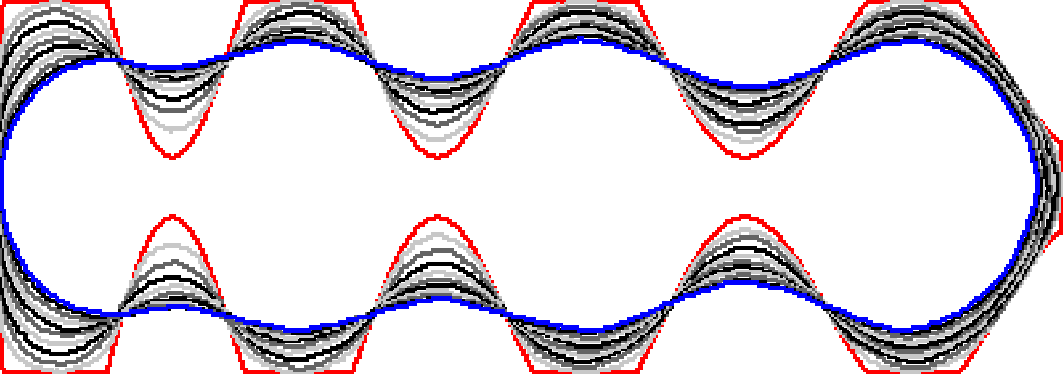
\includegraphics[scale=0.5]{figures/chapter6/faster-high-curvature/summary_flow.pdf}}\\%
%\subfloat[]{%
%		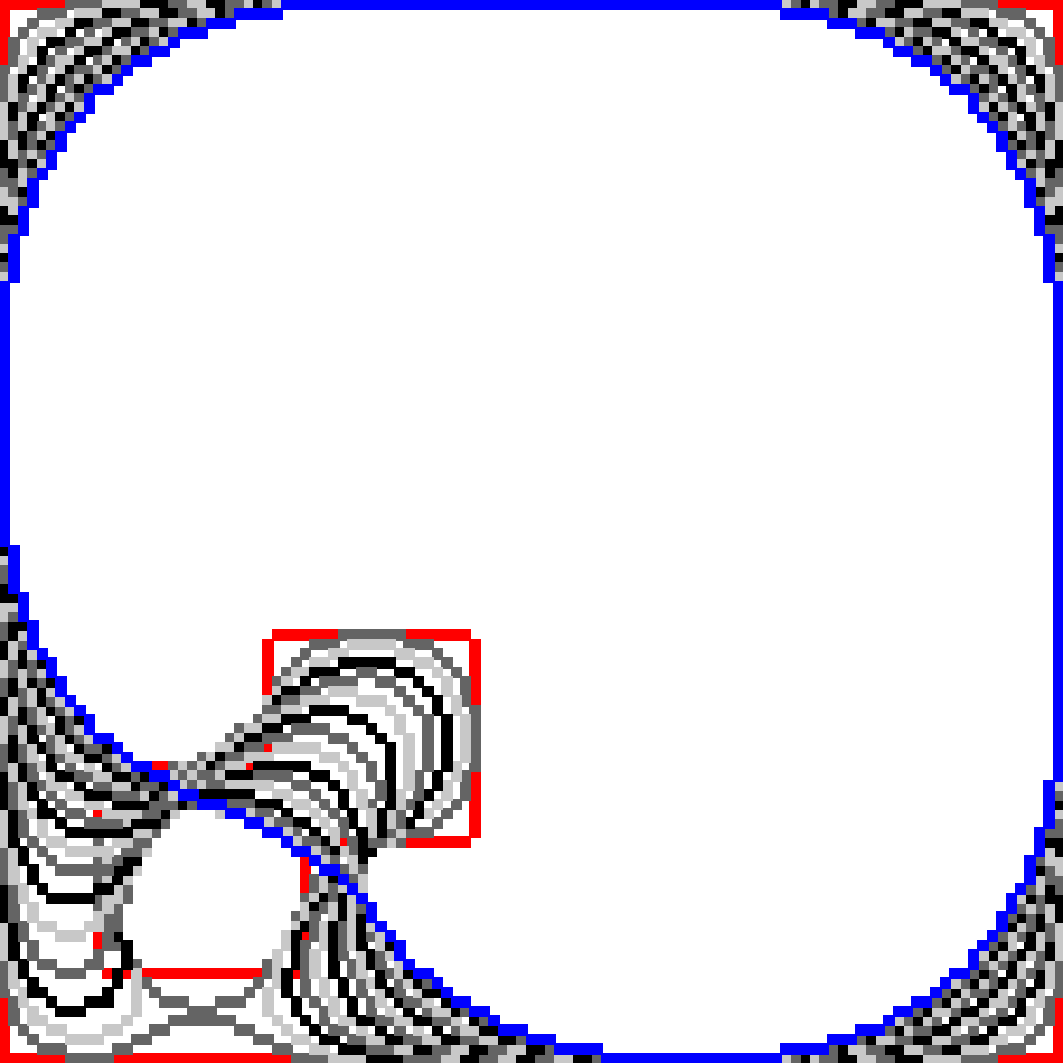
\includegraphics[scale=0.25]{figures/chapter6/fill-holes/summary_flow.pdf}}%%1
%\caption{High curvature regions evolves faster than lower ones (a). The flow can handle topological changes (b). }
%\label{fig:mx-speed-variation-hole-filling}
%\end{figure}


\section{Optimization method}

Let $f$ be a function of $n$ binary variables with unary and pairwise terms, i.e.

\begin{align*}
f(y_1,\cdots, y_n) = \sum_{j}{f_j(y_j)} + \sum_{j < k}{f_{j,k}(y_j,y_k)}.
\end{align*}

The function $f$ is submodular if and only if the following inequality holds for each pairwise term $f_{j,k}$ \cite{kolmogorov04whatenergies}:
\begin{align*}
  \quad f_{j,k}(0,0) + f_{j,k}(1,1) \leq f_{j,k}(0,1) + f_{j,k}(1,0).
\end{align*}

The energy $E_m$ is non-submodular and optimizing it is a difficult problem, which constrains us to use heuristics and
approximation algorithms. The QPBO method \cite{rother07qpbo} transforms the original problem in a max-flow/min-cut
formulation and yields a full optimal labeling for submodular energies. For non-submodular energies the method is
guaranteed to return a partial labeling with the property that the set of labeled variables is part of an optimal
solution. That property is called partial optimality.

In practice, QPBO can leave many pixels unlabeled. There exist two extensions to QPBO that alleviate this limitation:
QPBOI (improve) and QPBOP (probe). The first is an approximation method that is guaranteed to not increase the energy,
but loses the property of partial optimality. The second is an exact method which is reported to label more variables
than QPBO.

The percentage of unlabeled pixels by QPBOP for $E_1$ is quite high, but the percentage decreases to zero as we set $m$
equal to $r$. Therefore, we are more confident in taking the solution for values of $m$ close to $r$. However, the way it
varies across values of $m$ differs from shape to shape, as is illustrated in figure
\ref{fig:unlabeled-versus-iterations}. We also noticed that, for $m=r$, all the pixels were labeled, {which may
  indicate that $E_r$ is an easy instance of the general non-submodular energy $E_m$, but this remains to be
  proved. The number of pairwise terms in $E_r$ is roughly half of those in $E_1$ (see figure
  \ref{fig:ratio-pairwise-terms}).

  We have used QPBOI to solve $E_m$. Naturally, in the case where all pixels are labeled by QPBOP, QPBOI returns the
  same labeling as QPBOP.


%\begin{figure}
%\center
%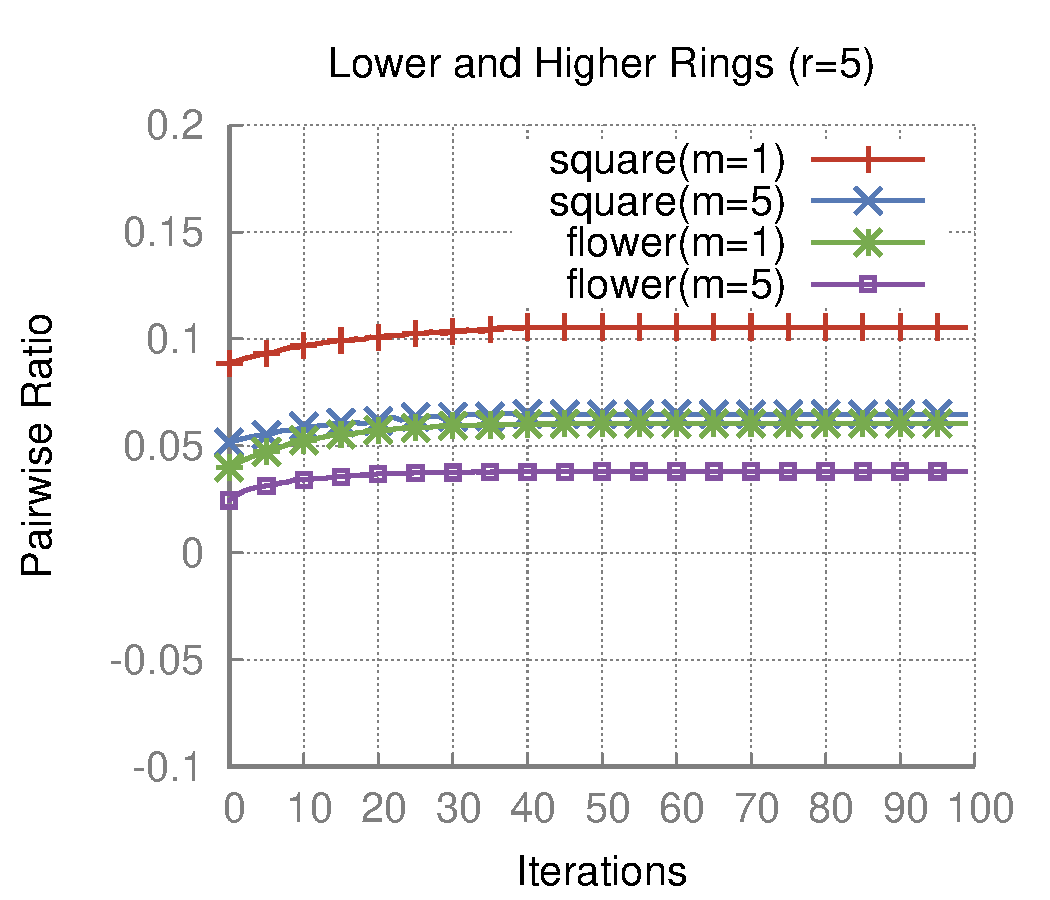
\includegraphics[scale=0.5]{figures/chapter6/pairwise-ratio/plot-pairwiseratio-lowerHigher-concavities-probe.pdf}
%\caption{We plot the ratio of pairwise terms among all $\binom{|X^{(i)}|}{2}$ combinations. The highest ring has roughly half the number of pairwise terms as the lowest ring.}
%\label{fig:ratio-pairwise-terms}
%\end{figure}


%\begin{figure}[]
%\center
%\begin{minipage}[b]{0.5\textwidth}
%\subfloat[]{ 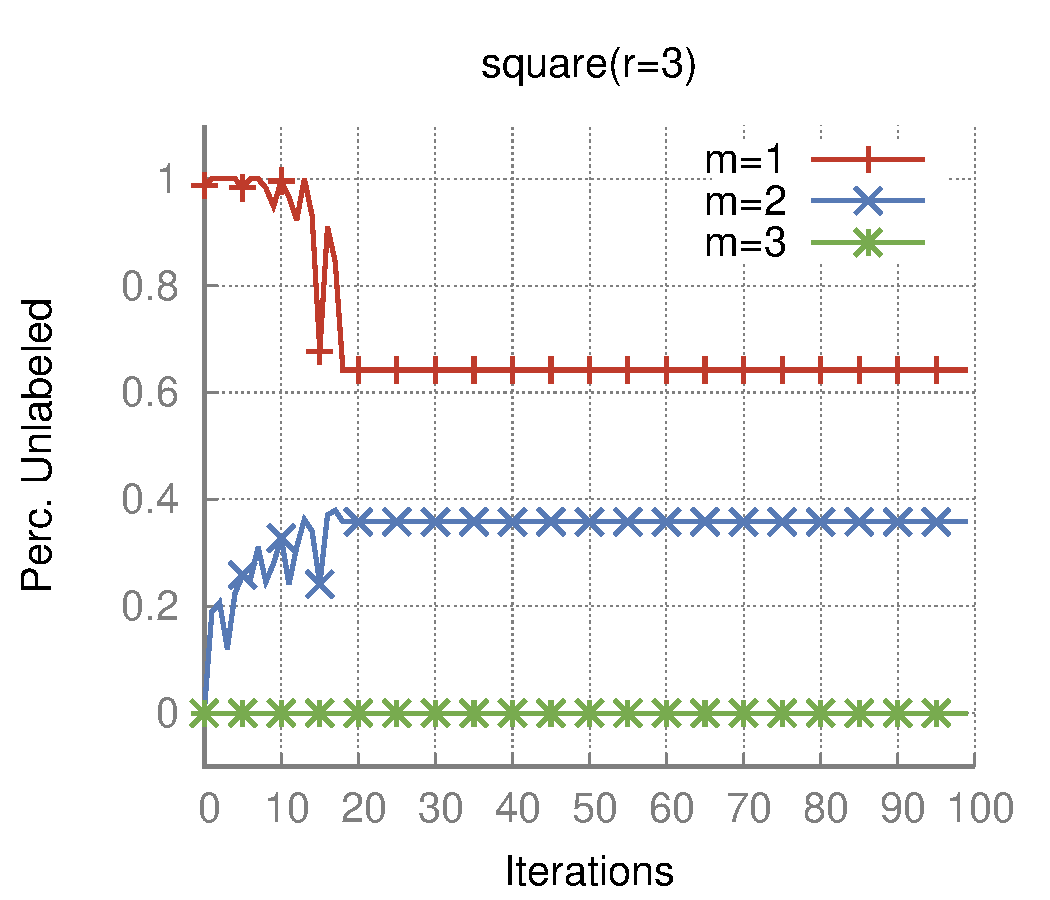
\includegraphics[scale=0.35]{figures/chapter6/unlabeled-iterations/radius-3/plot-model-square-concavities-probe.pdf}}\\%
%\subfloat[]{ 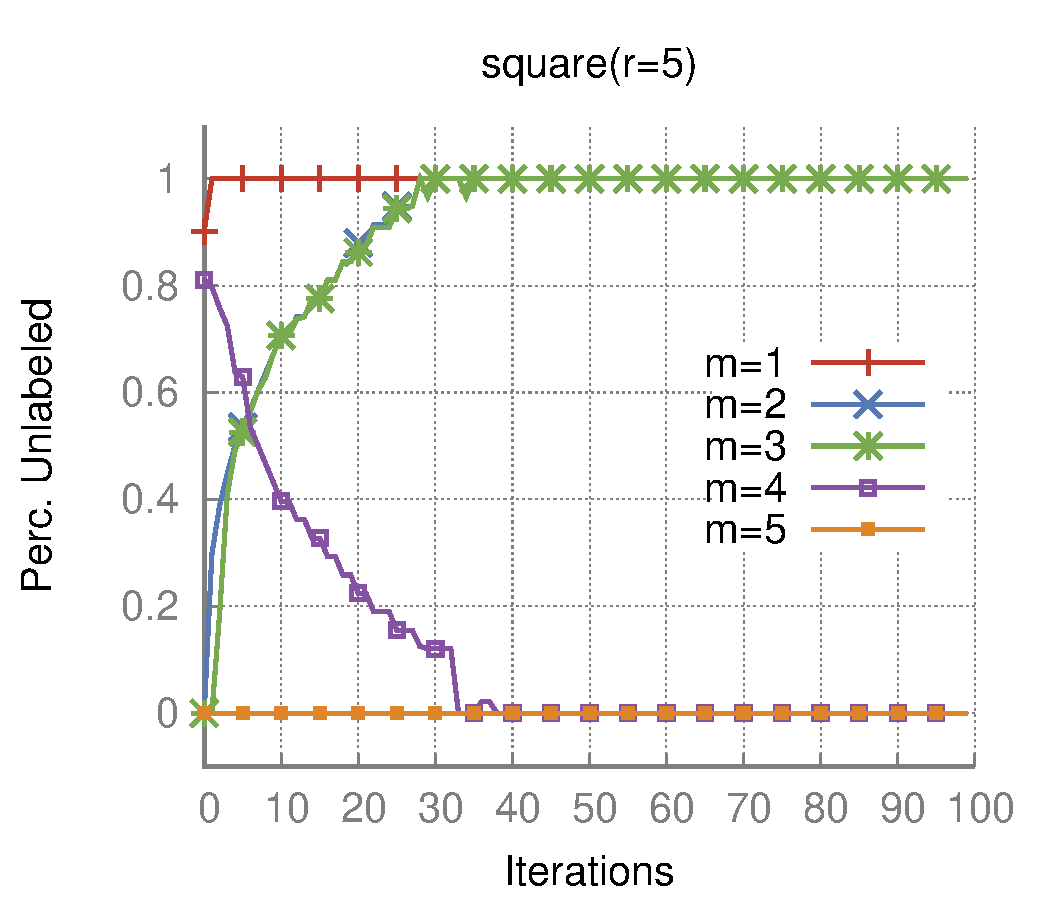
\includegraphics[scale=0.35]{figures/chapter6/unlabeled-iterations/radius-5/plot-model-square-concavities-probe.pdf}}\\%
%\subfloat[]{ 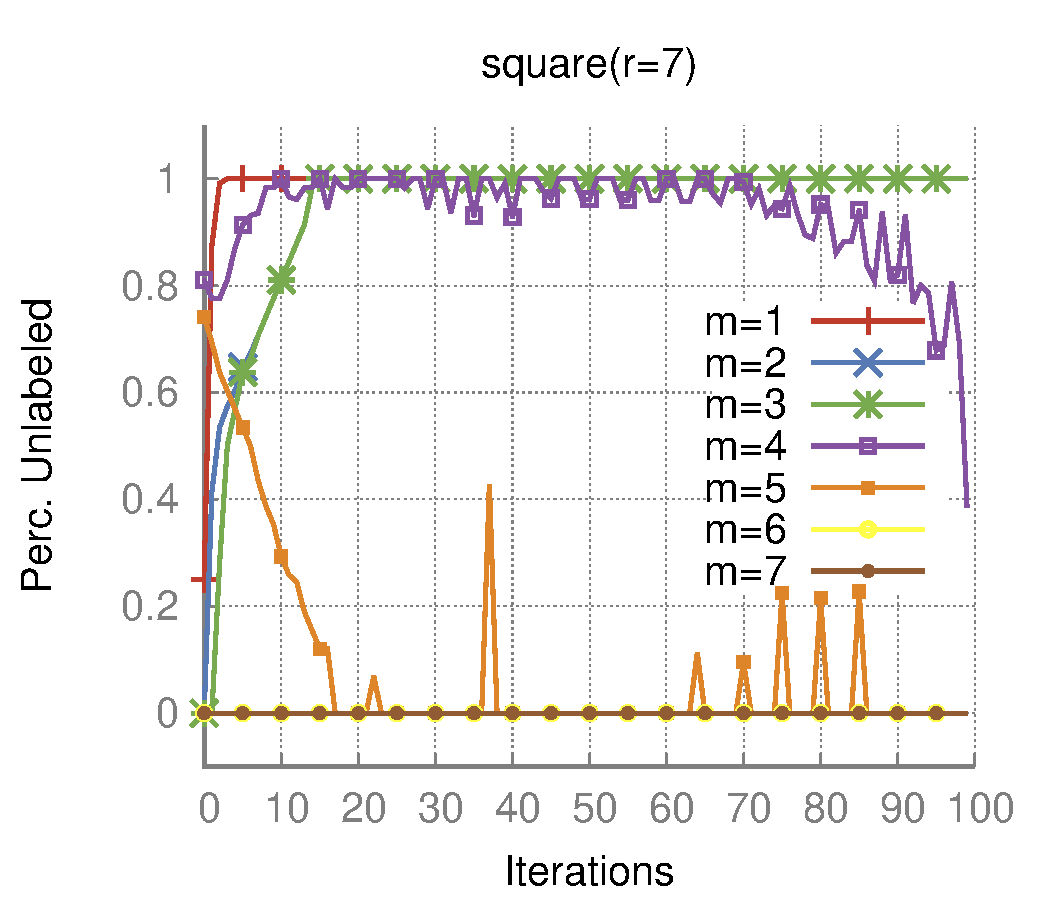
\includegraphics[scale=0.35]{figures/chapter6/unlabeled-iterations/radius-7/plot-model-square-concavities-probe.pdf}}%
%\end{minipage}%
%\begin{minipage}[b]{0.5\textwidth}
%\subfloat[]{ 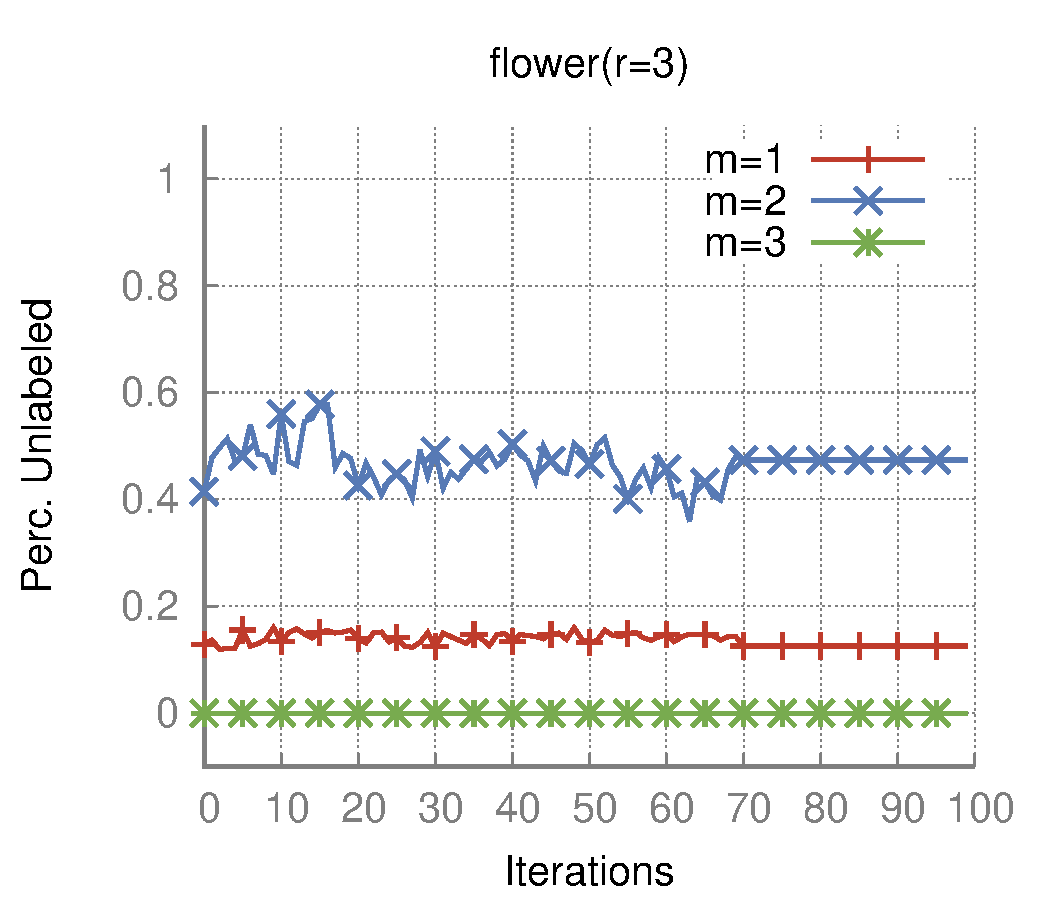
\includegraphics[scale=0.35]{figures/chapter6/unlabeled-iterations/radius-3/plot-model-flower-concavities-probe.pdf}}\\%
%\subfloat[]{ 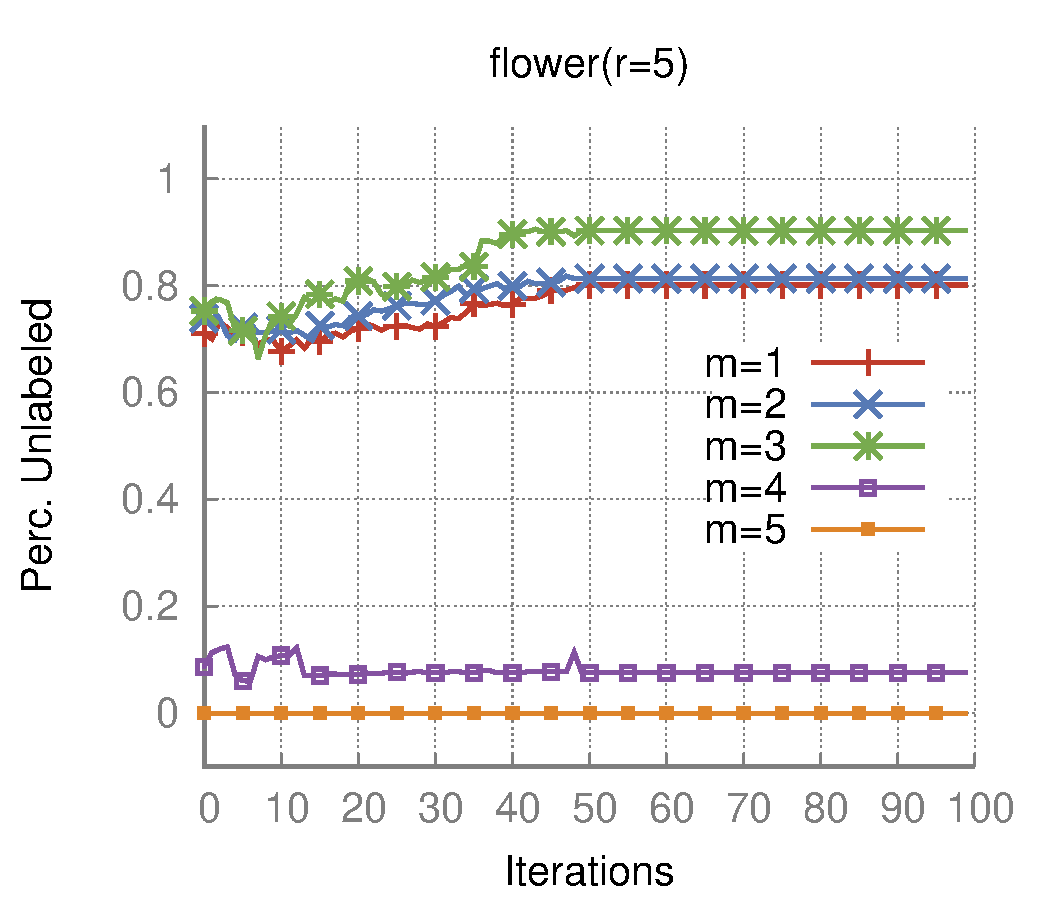
\includegraphics[scale=0.35]{figures/chapter6/unlabeled-iterations/radius-5/plot-model-flower-concavities-probe.pdf}}\\%
%\subfloat[]{ 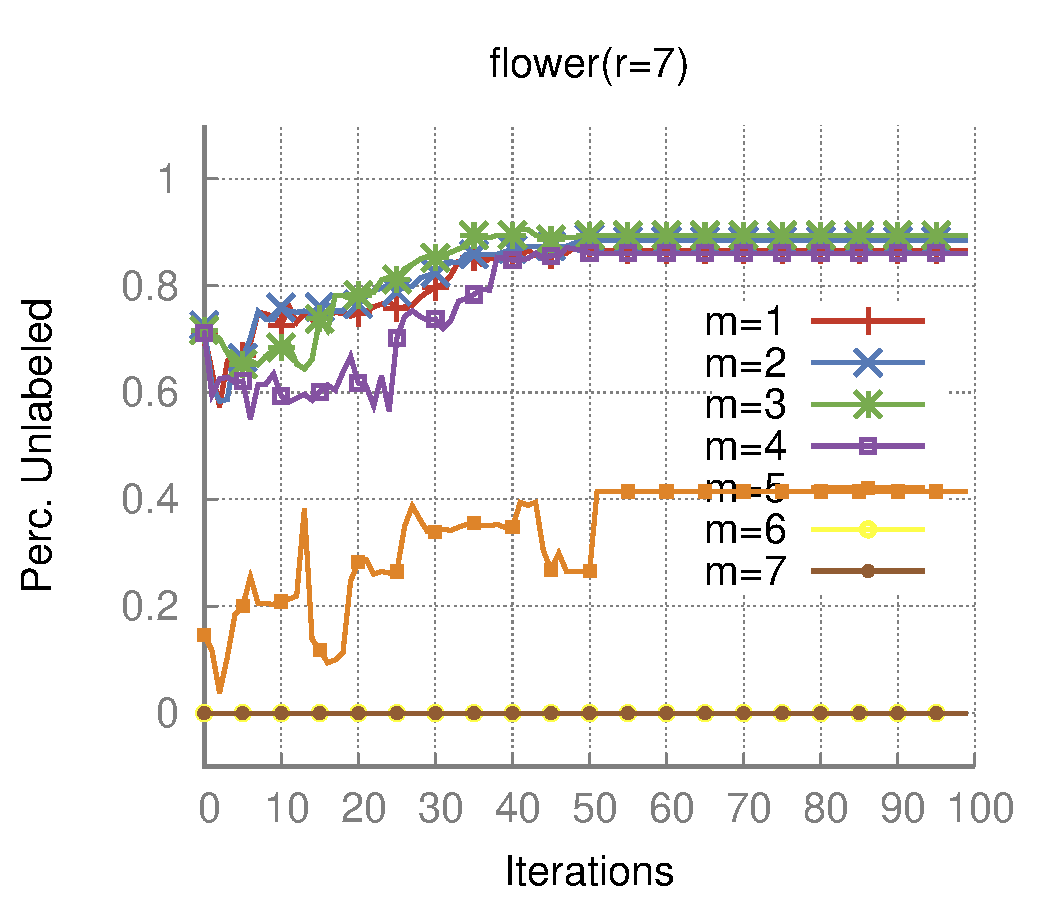
\includegraphics[scale=0.35]{figures/chapter6/unlabeled-iterations/radius-7/plot-model-flower-concavities-probe.pdf}}%
%\end{minipage}
%\caption{For each plot, we first produce shapes $\left\{ S^{(i)} \right\}$ executing DCE with $m=r$. Then, for each shape in $\left\{ S^{(i)} \right\}$, we execute one iteration of DCE for different values of $m$ and we count the unlabeled pixels. The number of unlabeled pixels by QPBOP remains high for lower values of $m$, and goes to zero when $m=r$. We observe the same behaviour for varying radius values.}
%\label{fig:unlabeled-versus-iterations}
%\end{figure}

